% \chapter{Theory of Beam Dynamics Relevant to the Large Hadron Collider}
\chapter{Relevant Theory of Beam Dynamics}
\label{chapter:Theory} % For referencing the chapter elsewhere, use \cref{chapter:Theory}

%----------------------------------------------------------------------------------------

The design, operation, performance, and safety of a particle accelerator depend on the study of beam dynamics.
This section provides an overview of the beam dynamics theories relevant to the material in this thesis, and more specifically beam optics.
For a more complete treatment of relevant accelerator physics the reader is best referred to textbooks by Wilson~\cite{BOOK:Wilson:Introcution_Particle_Accelerators}, Lee~\cite{BOOK:Lee:Accelerator_physics}, Wiedemann~\cite{BOOK:Wiedemann:Particle_Accelerator_Physics}, Minty and Zimmermann~\cite{BOOK:Minty:Measurements_Control_Charged_Particle_Beams}, Wolski~\cite{BOOK:Wolski:Beam_dynamics} or Chao~\cite{BOOK:Chao:Handbook_Accelerator_Physics_Engineering, BOOK:Chao:Collective_instabilities}.
Most of the material in this section can be found in the aforementioned literature, and when not in these works explicit references to the relevant content are given.

The chapter starts out with a description of linear dynamics and a parametrization of turn-by-turn motion in a circular accelerator.
It then moves on to aspects of non-linear dynamics and the use of normal form to obtain the non-linear motion, then follows with an introduction to betatron coupling and ends with a discussion of luminosity.

%----------------------------------------------------------------------------------------

\section{Linear Beam Dynamics}
\label{section:linear_beam_dynamics}

The linear dynamics of an accelerator are, mainly, the endeavor to bend and focus particle beams to confine them within the machine's aperture.

\subsection{Transport and Guiding of Charged Particles}
\label{subsection:transport_and_guiding_of_charged_particles}

To force the beam's particles into a closed trajectory, they are subjected to magnetic fields that deflect their trajectories.
The force exerted onto the beam is the Lorentz force \(F_{L}\) given by the equation:

\begin{equation}
    \vec{F_L} = \dfrac{d\vec{p}}{dt} = q (\vec{E} + \vec{v} \times \vec{B}) \text{ ,}
    \label{equation:lorentz_force}
\end{equation}
where \(\vec{p}\) is the particle momentum, \(q\) the particle charge, \(\vec{E}\) the electric field, \(\vec{v}\) the particle velocity and \(\vec{B}\) the magnetic field.
In most accelerators, including the LHC, the particles' speed is close to the celerity of light \(c\) and the force from the magnetic field is significantly stronger than that produced by the electric field for realistic values of \(\vec{E}\) and \(\vec{B}\).
As a result, while electric fields are used for acceleration, in high energy particle accelerators magnetic fields are typically used to guide particles.
The guiding magnetic field can be expanded into a series of multipolar fields, for instance here in the horizontal plane:

\begin{align}
    B_{y} = 
    \tikz[baseline]{
        \node[draw=red,rounded corners,anchor=base] (m1)
        {\(\displaystyle B_{y0}\)};
        \node[below of=m1] (l1) {dipole};
        \draw[-,red] (l1) -- (m1);
    }
    +
    \tikz[baseline]{
        \node[draw=red,rounded corners,anchor=base] (m2)
        {\(\displaystyle \frac{dB_{y}}{dx} x\)};
        \node[below of=m2] (l2) {quadrupole};
        \draw[-,red] (l2) -- (m2);
    }
    +
    \tikz[baseline]{
        \node[draw=red,rounded corners,anchor=base] (m3)
        {\(\displaystyle \frac{1}{2!} \frac{d^2B_{y}}{dx^2} x^2\)};
        \node[below of=m3] (l2) {sextupole};
        \draw[-,red] (l2) -- (m3);
    }
    +
    \tikz[baseline]{
        \node[draw=red,rounded corners,anchor=base] (m4)
        {\(\displaystyle \frac{1}{3!} \frac{d^3B_{y}}{dx^3} x^3\)};
        \node[below of=m4] (l2) {octupole};
        \draw[-,red] (l2) -- (m4);
    }
    + \ldots
    \label{equation:magnetic_field_expansion}
\end{align}

Bending forces are supplied by dipole magnets with a magnetic field perpendicular to the beam trajectory, while focusing is typically performed with the use of quadrupole magnets.
Higher orders belong to the non-linear dynamics and will be discussed later on.
\Cref{figure:frenet_serret_system} illustrates the Frenet-Serret coordinate system traditionally used in linear beam dynamics.

\begin{figure}[!htb]
    \begin{center}
    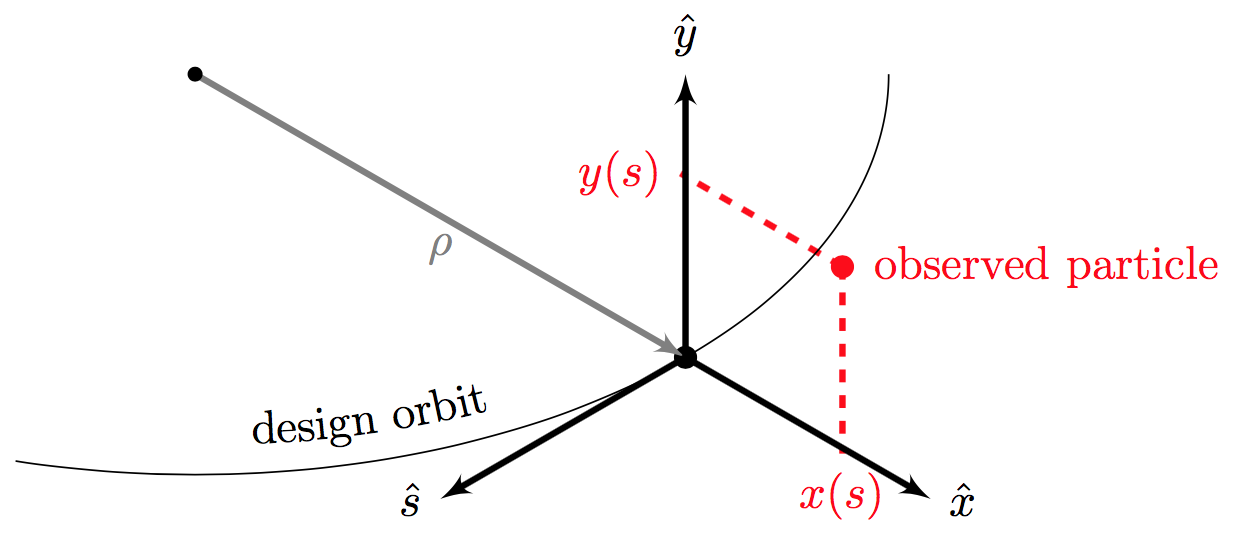
\includegraphics[width = 0.8\linewidth]{Figures/Beam_Dynamics_Theory/Frenet_Serret_Coordinate_System.png}
    \caption{The Frenet-Serret coordinate system used in accelerator physics. Here \(\hat{x}\), \(\hat{y}\), and \(\hat{s}\) form the right-handed orthogonal basis, while \(\rho\) is the local bending radius.}
    \label{figure:frenet_serret_system}
    \end{center}
\end{figure}

The coordinate system travels longitudinally with the particle, along a reference trajectory defined by an ideal, or \intro{synchronous}, particle.
The longitudinal curvilinear coordinate is \(s\), and denotes the position of the particle along the ideal orbit with respect to an arbitrary initial point at \(s = 0\).
One can define a local radius of curvature, \(\rho(s)\), which depends on the local magnetic field \(\vec{B}\) and varies along ring.
The transverse phase space is defined by \((x, x^{\prime}, y, y^{\prime})\), where \(x\) and \(y\) are a particle's coordinates in the transverse planes relative to the reference trajectory.
The \(x^{\prime}\) and \(y^{\prime}\) coordinates are \intro{divergent angles}, with the prime indicating differentiation with respect to \(s\).
\break

In the linear regime, magnetic dipoles define the ideal orbit for a particle of \intro{reference momentum} \(p_0\).
This ideal orbit goes through the magnetic center of all elements in the machine to close back on itself after a revolution, and is called the \intro{closed orbit}.
In practice the real closed orbit will deviate from the ideal designed orbit due to various effects such as dipolar field errors.
Particles within the beam are distributed in amplitude and oscillate around the closed orbit, which corresponds to the path of a particle with zero amplitude within the beam, because of focusing forces. 
This is illustrated in \cref{figure:design_vs_particle_orbit} where a conceptualized design orbit is shown in blue and an actual particle orbit in red.

\begin{figure}[!htb]
    \begin{center}
    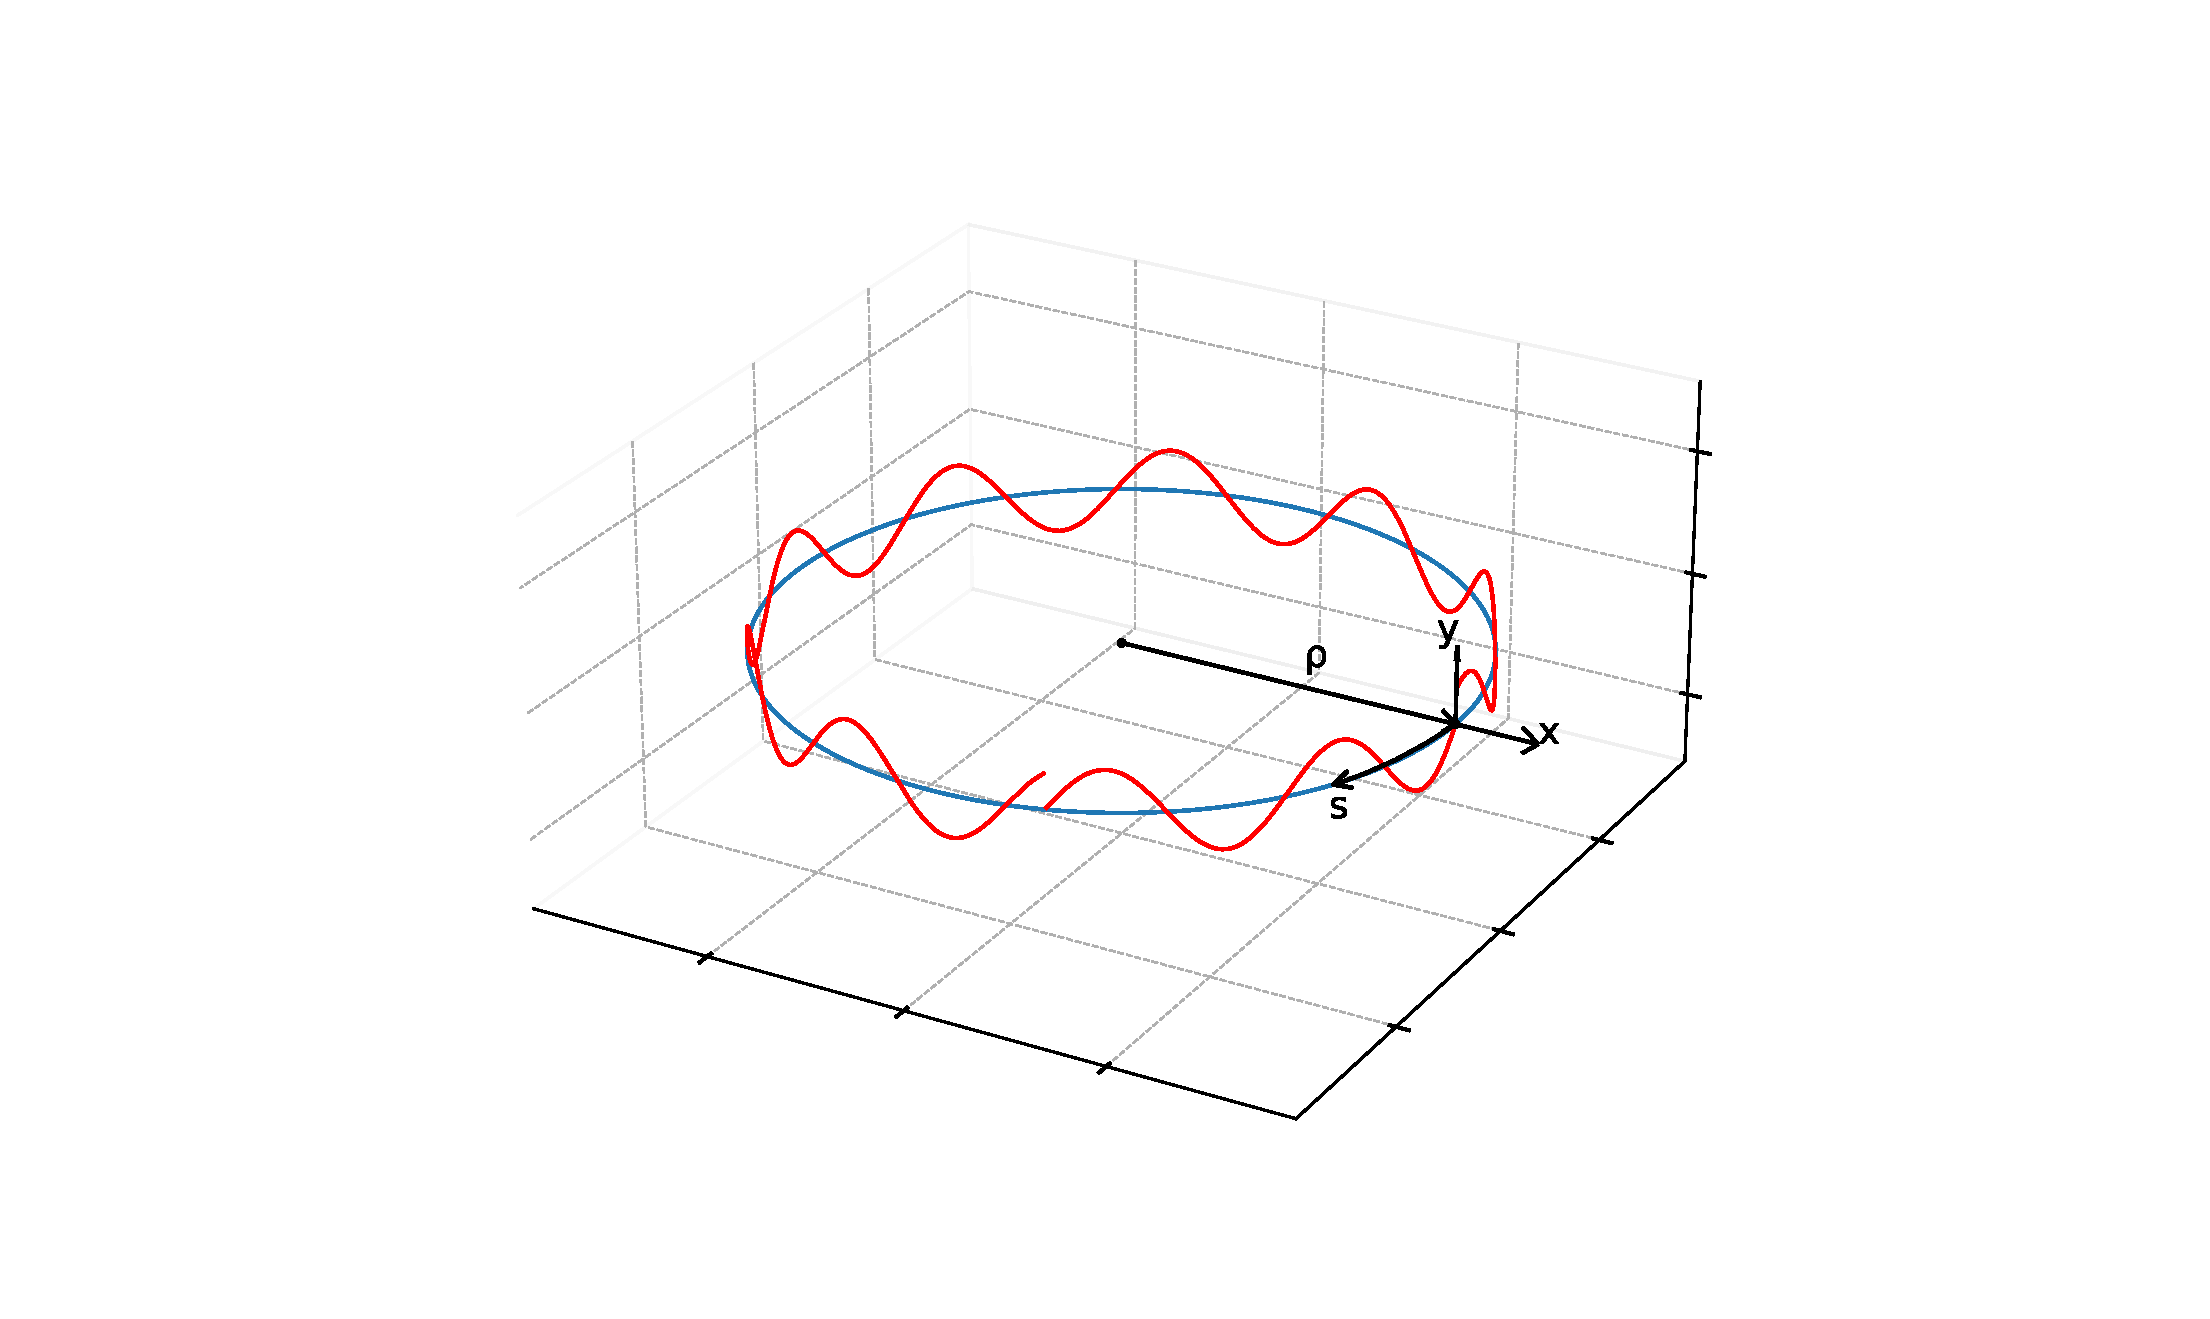
\includegraphics[width = 0.9\linewidth]{Figures/Beam_Dynamics_Theory/design_vs_particle_orbit.pdf}
    \caption{Illustration of a design closed orbit (blue) and a particle orbit oscillating around it (red).}
    \label{figure:design_vs_particle_orbit}
    \end{center}
\end{figure}

Focusing forces are typically provided by magnetic quadrupoles: a quadrupolar field acting on a charged particle displaced from the closed orbit will provide a restoring (focusing) force proportional to the displacement in one transverse plane, while simultaneously providing a diverging (defocusing) force in the other. 
As a convention, a quadrupole focusing in the horizontal plane and defocusing in the vertical one is referred to as a \intro{focusing quadrupole}. 
Respectively, a quadrupole defocusing in the horizontal plane but focusing in the vertical one is referred to as a \intro{defocusing quadrupole}.

A net focusing effect in both planes can be obtained with a setup of quadrupoles of alternating polarity in equal distance, a widely used configuration named the \intro{FODO cell}.
A schematic of a FODO cell is shown in \cref{figure:fodo_cell_schematic}, and \cref{figure:dipole_quadrupole_fields} illustrates magnetic fields in an idealized dipole and quadrupole.

\begin{figure}[!htb]
    \begin{center}
    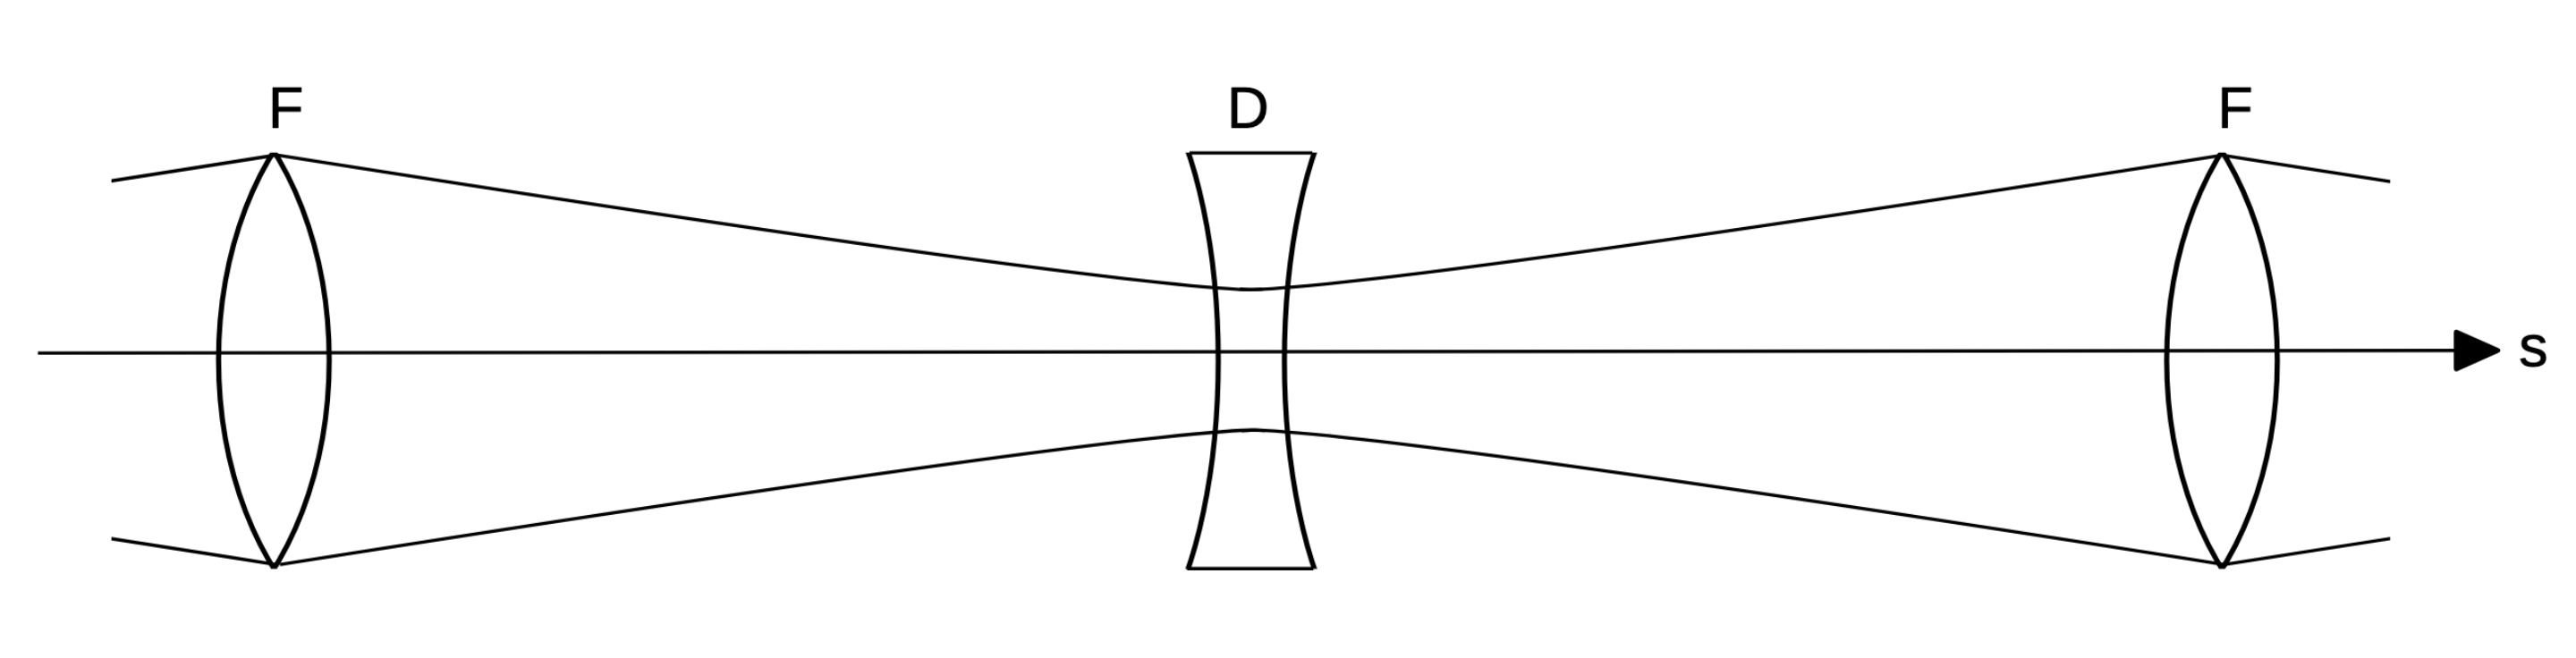
\includegraphics[width = 0.8\linewidth]{Figures/Beam_Dynamics_Theory/fodo_cell_schematic.png}
    \caption{Schematic of a FODO cell. A focusing quadrupole is denoted with an F while a defocusing one is denoted with a D.}
    \label{figure:fodo_cell_schematic}
    \end{center}
\end{figure}

For each magnet applying a field \(B\) one can define the \intro{magnetic rigidity}, which is an indication of the field's ability to alter a particle's course based on its charge \(q\) and momentum \(p\), as:

\begin{equation}
    B \rho = \frac{p}{q} \text{ .}
    \label{equation:magnetic_rigidity}
\end{equation}

\begin{figure}[!hbt]
    \begin{center}
    \begin{subfigure}[b]{0.45\textwidth}
        \begin{center}
        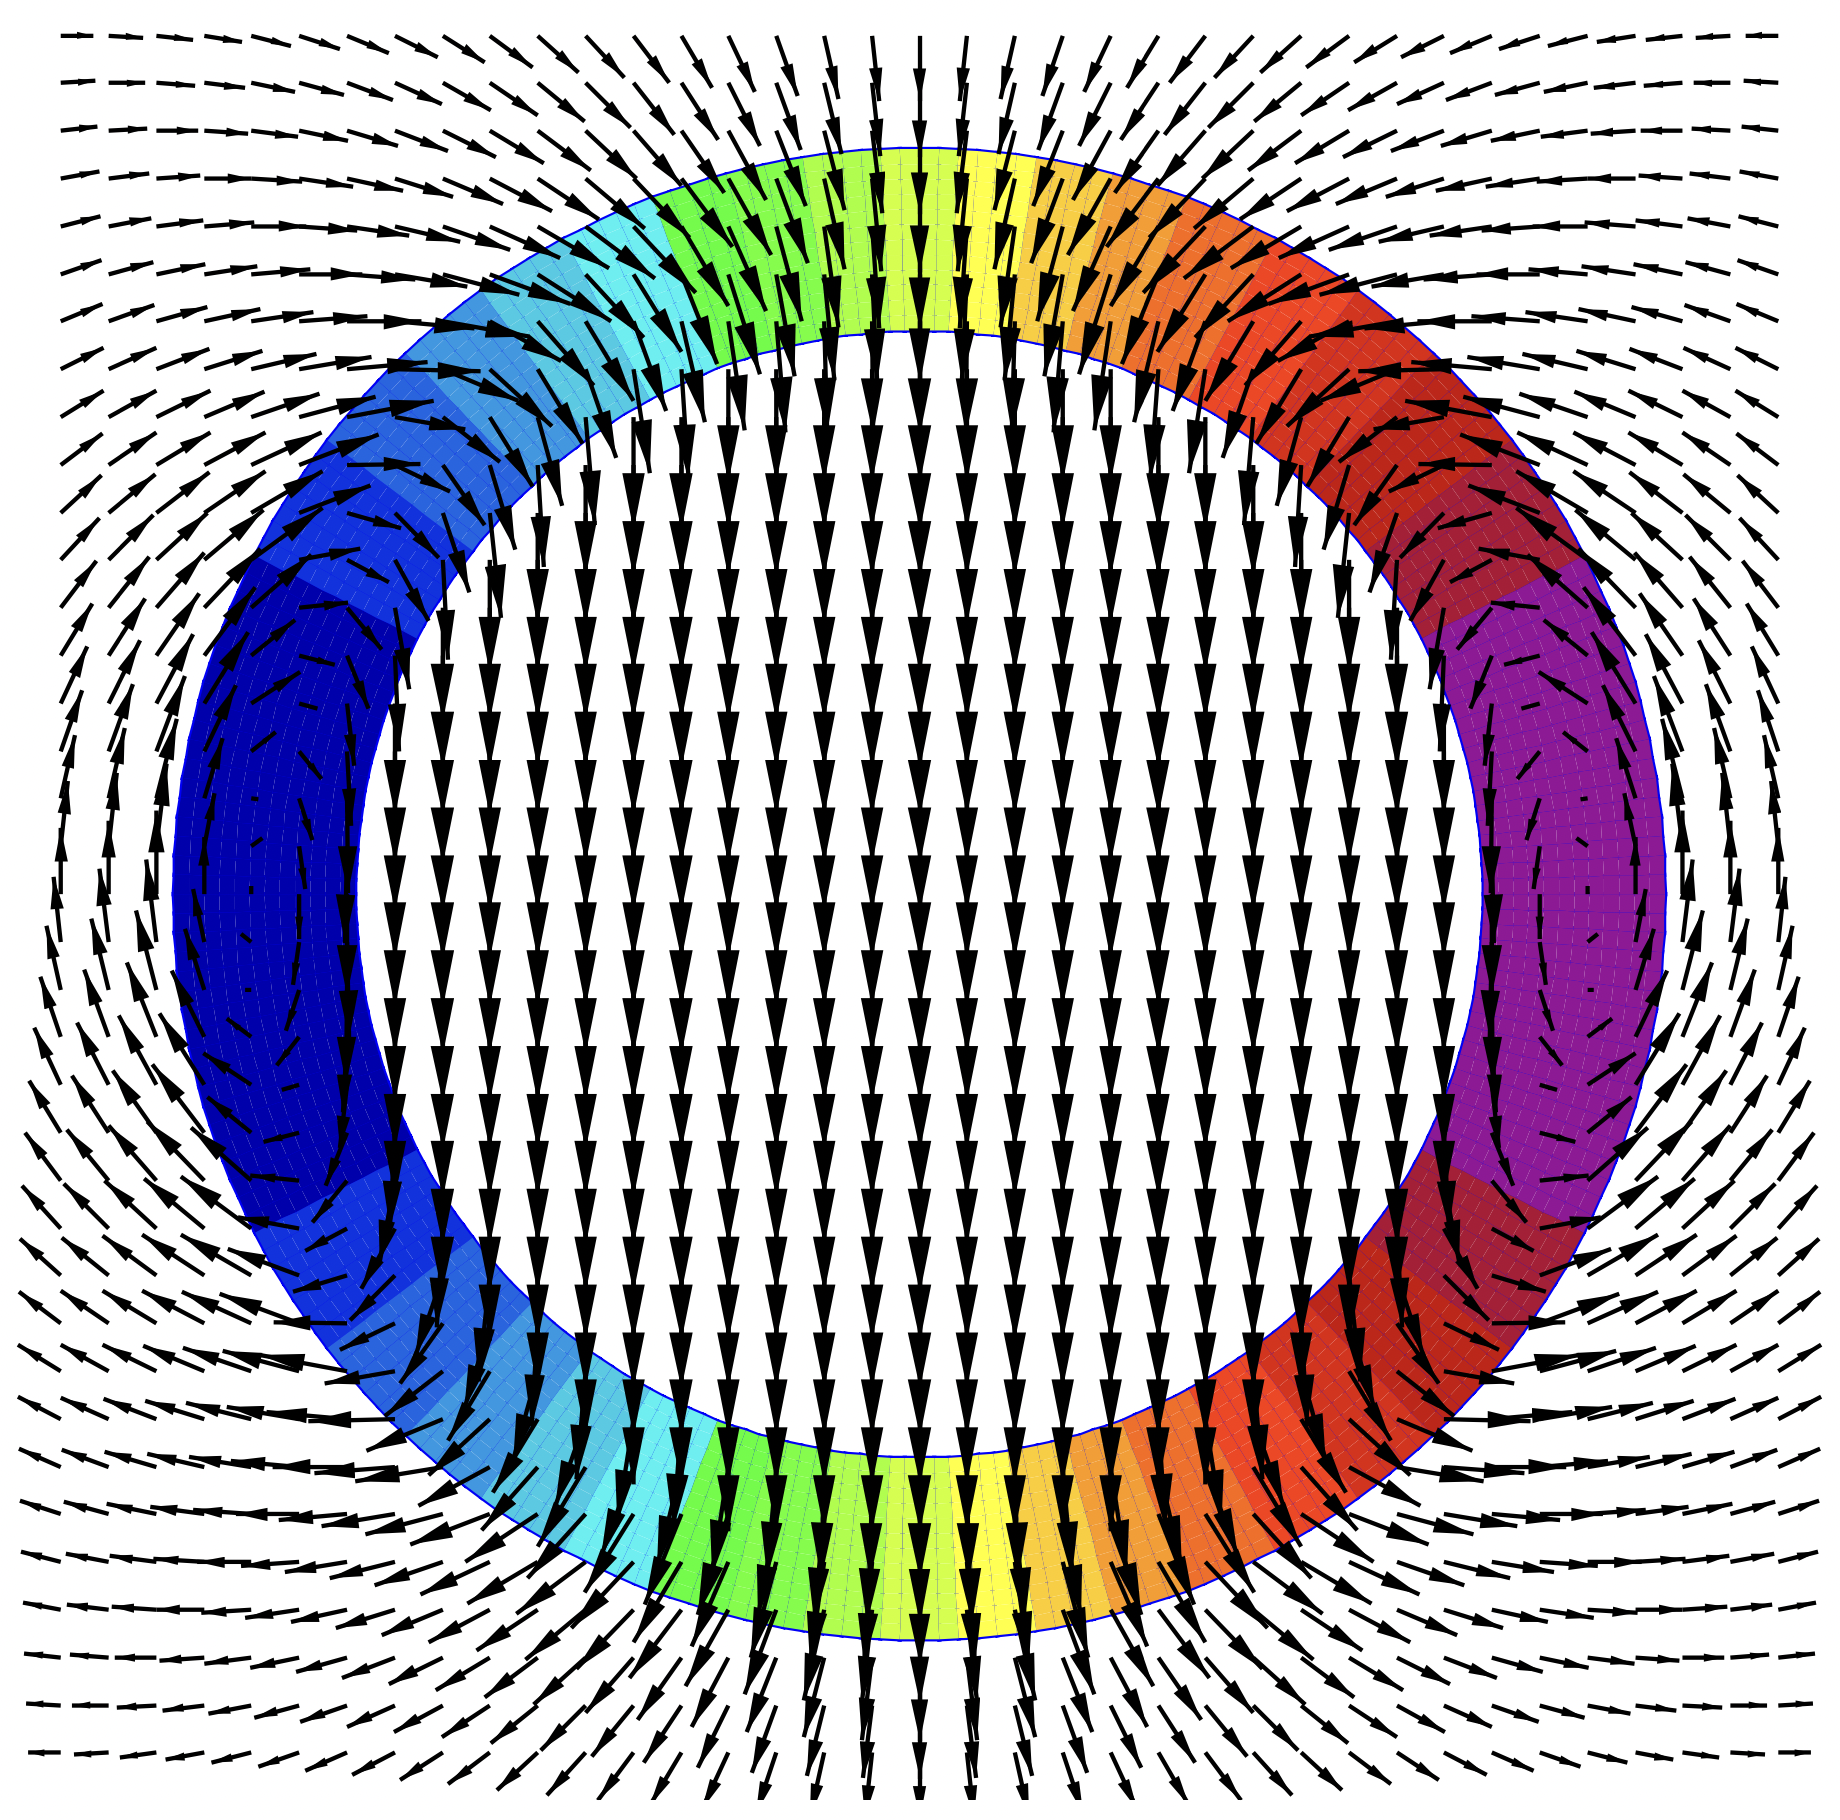
\includegraphics[width=\textwidth]{Figures/Beam_Dynamics_Theory/ideal_dipole_cos_theta.png}
        \caption{Ideal dipole.}
        \label{fig:ideal_dipole}
        \end{center}
    \end{subfigure}
    \hfill
    \begin{subfigure}[b]{0.45\textwidth}
        \begin{center}
        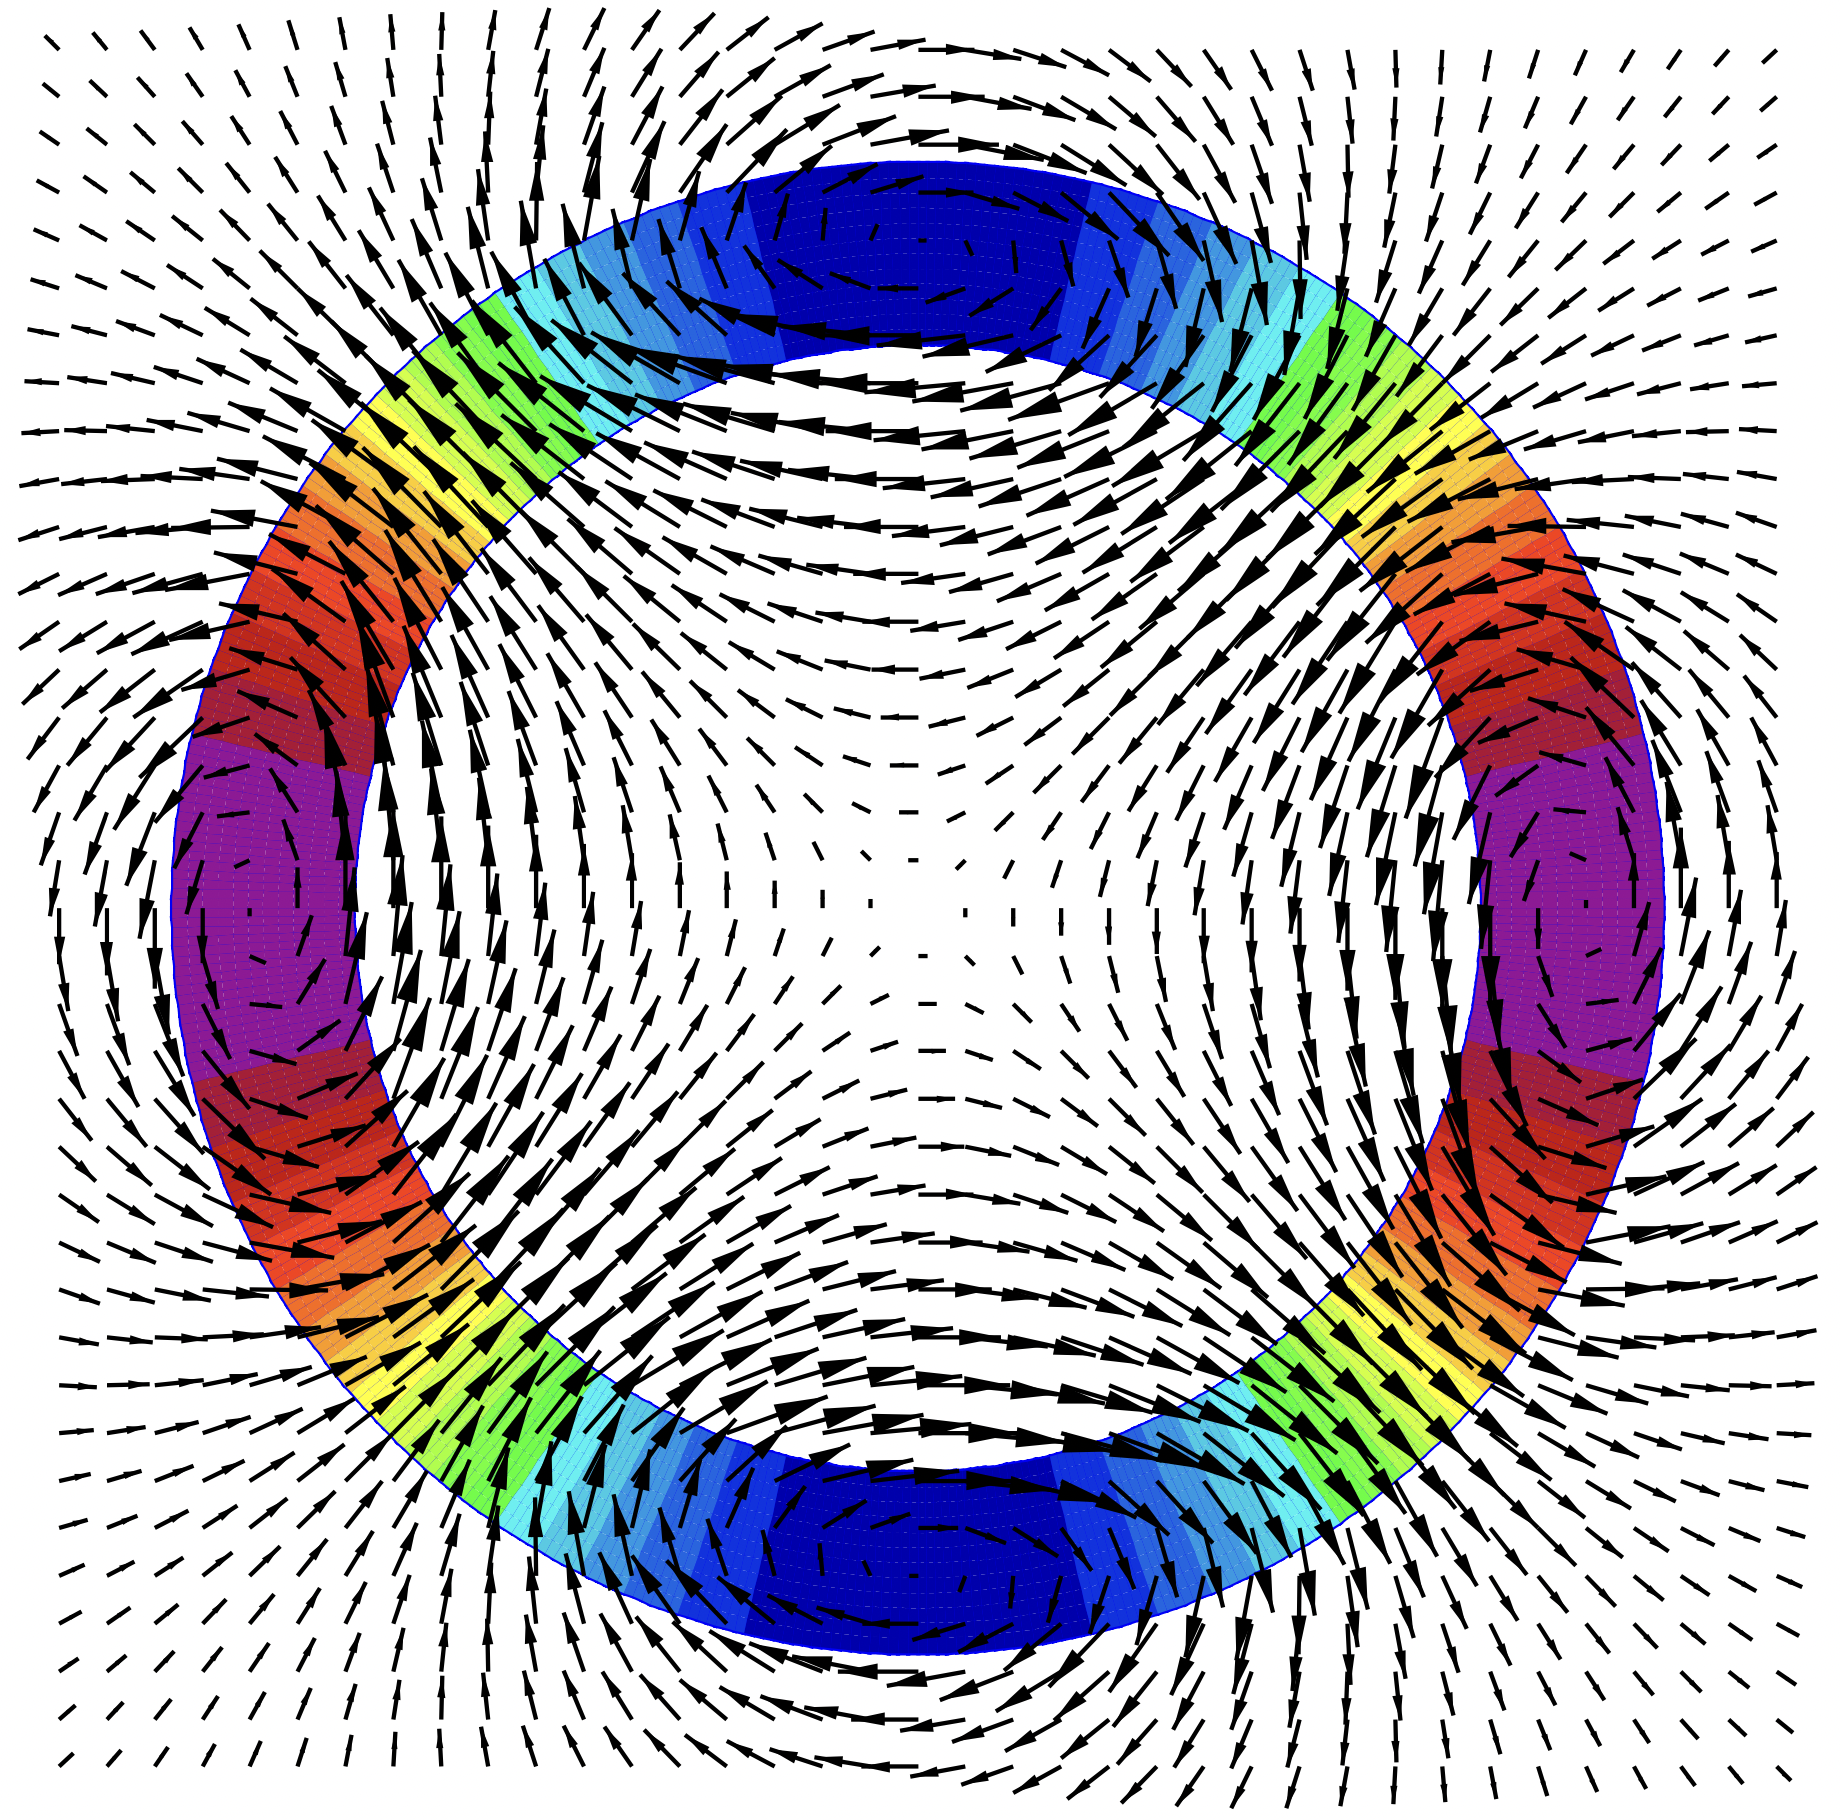
\includegraphics[width=\textwidth]{Figures/Beam_Dynamics_Theory/ideal_quadrupole_cos_2theta.png}
        \caption{Ideal quadrupole.}
        \label{fig:ideal_quadrupole}
        \end{center}
    \end{subfigure}
    \caption{Magnetic fields and forces in an idealized dipole and quadrupole, with a \(\cos(\theta)\) and \(\cos(2\theta)\) current distribution in the circular coil, respectively. Current in the dipole and quadrupole coils are indicated in color. These visuals were taken from \cite{CERN:Russenschuck:CAS_Design_Magnets}.}
    \label{figure:dipole_quadrupole_fields}
    \end{center}
\end{figure}

\subsection{Equations of Motion and Twiss Parameters}
\label{subsection:equations_of_motion_and_twiss_parameters}

The focusing from quadrupoles in a circular accelerator such as the LHC is periodic in \(s\), with a period of at most the circumference of the machine.
Assuming the existence of a \kl{closed orbit}, the transverse motion of a single particle in a synchrotron with a periodic lattice is described by Hill's equation:

\begin{equation}
    z^{\prime \prime}(s) + K_z(s) z(s) = 0; \quad z = x, y; \quad z^{\prime} = \dfrac{dz}{ds} \text{ ,}
    \label{equation:hill_equation}
\end{equation}
where \(K_z\) represents the focusing effect of dipoles and quadrupoles in the transverse planes, and varies with \(s\) as it is dictated by magnetic elements traversed by particles.
It can be expressed according to:

\begin{equation}
	\begin{aligned}
		K_x(s) &= \frac{1}{\rho^2} - k_1(s) \text{ ,} \\
    	K_y(s) &= k_1(s) \text{ ,}
	\end{aligned}
    \label{equation:transverse_focusing_strengths}
\end{equation}
where \(k_1(s)\) is the normalized quadrupole strength.
A \kl{focusing quadrupole} has a \(K > 0\), a \kl{defocusing quadrupole} has \(K < 0\), and a drift space has \(K = 0\).
The term \(\left(1 / \rho^2\right)\) in the horizontal component arises from the weak focusing caused by dipoles.

In the material below, \(z\) will be used to denote either \(x\) or \(y\), the rules applying to both similarly.
According to the theorem of Floquet~\cite{BOOK:Lee:Accelerator_physics}, the solution with periodic boundary conditions to Hill’s equation takes the form of \cref{equation:hill_solution}:

\begin{equation}
    \begin{aligned}
        z(s)          &= \sqrt{\beta_{z}(s) \varepsilon_{z}} \cos \left( \phi_{z}(s) + \phi_{z,0} \right) \text{ ,} \\
        z^{\prime}(s) &= -\sqrt{\frac{\varepsilon_z}{\beta_z(s)}} \left( \sin \left(\phi_z(s) + \phi_{z, 0} \right) + \alpha(s) \cos \left( \phi_z(s) + \phi_{z, 0} \right) \right) \text{ .}
    \end{aligned}
    \label{equation:hill_solution}
\end{equation}

These equations describe a harmonic oscillation in the transverse planes.
Here \(\varepsilon_z\) is the \intro{geometric emittance} of a particle and is a constant of the motion at a given energy. 
\(\phi_z(s)\) is the \intro{phase advance} and \(\alpha_z(s)\) is the \intro{alpha-function}.
\(\beta_z(s)\) is the \intro{beta-function} and represents the fluctuation of the oscillation envelope around the ring: it describes the transverse position dependent amplitude of the oscillation and has the dimension of a length.
In particle colliders such as the LHC the \(\beta\)-functions at the Interaction Points (IP), where the beams are made to collide, are commonly referred to as \(\beta_z^{\ast}\).
The solution of Hill's equation can also be written in matrix form as:

\begin{equation}
    \left(
        \begin{array}{c}
            z(s) \\
            z^{\prime}(s)
        \end{array} \right) = \mathrm{M} \left( 
        \begin{array}{c}
            z(0) \\
            z^{\prime}(0)
    \end{array} \right) \text{ .}
    \label{equation:hill_solution_matrix}
\end{equation}

In this form, which makes the assumption that the magnetic field of an element is constant along the longitudinal direction, M is called a \intro{transfer matrix}. 
Below are the transfer matrices corresponding to a drift space, \(\mathrm{M_{drift}}\), a dipole, \(\mathrm{M_{dip.}}\), a focusing quadrupole, \(\mathrm{M_{foc. quad.}}\), and a defocusing quadrupole \(\mathrm{M_{defoc. quad.}}\), respectively:

\begin{equation}
    \mathrm{M_{drift}} = \left(
        \begin{array}{ll}
            1 & L \\
            0 & 1
    \end{array} \right) \text{ ,}
    \label{equation:drift_transfer_matrix}
\end{equation}

\begin{equation}
    \mathrm{M_{dip.}} = \left(
        \begin{array}{cc}
            \cos \theta                          & \rho \sin \theta \\
            - \sin \left( \theta / \rho \right)  & \cos \theta
    \end{array} \right) \text{ ,}
    \label{equation:dipole_transfer_matrix}
\end{equation}

\begin{equation}
    \mathrm{M_{foc. quad.}} = \left(
        \begin{array}{cc}
            \cos \left( \sqrt{k_1} L \right)             & \frac{1}{\sqrt{k_1}} \sin \left( \sqrt{k_1} L \right) \\
            -\sqrt{k_1} \sin \left( \sqrt{k_1} L \right) & \cos \left( \sqrt{k_1} L \right)
    \end{array} \right) \text{ ,}
    \label{equation:focusing_quad_transfer_matrix}
\end{equation}

\begin{equation}
    \mathrm{M_{defoc. quad.}} = \left(
        \begin{array}{cc}
            \cosh \left( \sqrt{\abs{k_1}} L \right)                 & \frac{1}{\sqrt{\abs{k_1}}} \sinh \left( \sqrt{\abs{k_1}} L \right) \\
            \sqrt{\abs{k_1}} \sinh \left( \sqrt{\abs{k_1}} L \right) & \cosh \left( \sqrt{\abs{k_1}} L \right)
    \end{array} \right) \text{ ,}
    \label{equation:defocusing_quad_transfer_matrix}
\end{equation}
where \(L\) is the element length and \(\theta = L / \rho\) is the bending angle of the dipole.
The transfer matrix of a group of elements is obtained by multiplying the transfer matrices of all individual elements.
For example, the transfer matrix corresponding to the FODO cell of \cref{figure:fodo_cell_schematic} is:

\begin{equation}
    \mathrm{M_{FODO}} = \mathrm{M_{foc. quad.}} \cdot \mathrm{M_{drift}} \cdot \mathrm{M_{defoc. quad.}} \cdot \mathrm{M_{drift}} \text{ .}
    \label{equation:fodo_transfer_matrix}
\end{equation}

For a complete machine with hundreds to thousands of elements, the maps of linear elements can still be combined to obtain the coordinates of a particle after a full revolution.
This specific transfer map is called the \intro{one-turn map} and fully describes the linear evolution of a particle's coordinates over one revolution of the accelerator.
It can be expressed as:

\begin{equation}
    \mathrm{M_{OTM}} = \mathrm{M_N} \cdot \mathrm{M_{N-1}} \cdot \ldots \cdot \mathrm{M_2} \cdot \mathrm{M_1} \text{ ,}
    \label{equation:one_turn_map}
\end{equation}
where \(\mathrm{M_i}\) is the transfer matrix of the \(i\)th element in the machine.
The transformation of coordinates over a revolution is then given by:

\begin{equation}
    \left(
        \begin{array}{c}
            z \\
            z^{\prime}
        \end{array} \right)_{s_0 + C} = \mathrm{M_{OTM}} \cdot \left( 
        \begin{array}{c}
            z \\
            z^{\prime}
    \end{array} \right)_{s_0} \text{ .}
    \label{equation:one_turn_coordinates_transformation}
\end{equation}

The phase advance \(\phi_z(s)\) mentioned above corresponds to the difference of the betatron phase functions at two points, typically also taken with respect to an arbitrary initial point at \(s = 0\).
The phase advance between two points at longitudinal positions \(s_1\) and \(s_2\) in the lattice is defined as:

\begin{equation}
    \phi_{s_1 \rightarrow s_2} = \phi(s_{2}) - \phi(s_{1}) = \int_{s_{1}}^{s_{2}} \frac{1}{\beta(s)} ds \text{ .}
    \label{equation:phase_advance_definition}
\end{equation}

As particles go around the ring, they oscillate around the closed orbit within an enveloppe defined by the \(\beta\)-functions and the emittance.
The number of these so-called \intro{betatron oscillations} per revolution is the \intro{tune} \(Q_u\).
The tune is defined in \cref{equation:tune_definition}, where \(\Delta \phi_{x, y}\) is the total betatron phase advance of a particle over a full circumference:

\begin{equation}
    Q_z = \frac{1}{2 \pi} \Delta \phi_z = \frac{1}{2 \pi} \oint_C \dfrac{ds}{\beta_z (s)} \text{ .}
    \label{equation:tune_definition}
\end{equation}

The \(\alpha\)-function is defined via the derivative of the \(\beta\)-function by:

\begin{equation}
    \alpha_z(s) = - \frac{1}{2} \beta^{\prime}_z(s) \text{ .}
    \label{equation:alpha_function}
\end{equation}

Similarly to the \(\beta\)-function, the \intro{gamma-function} \(\gamma_u(s)\) describes the envelope of oscillations in \(x^{\prime}\) and \(y^{\prime}\).
Both quantities are related by the \(\alpha\)-function according to:

\begin{equation}
    \gamma_z(s) = \frac{1 + \alpha_z^2(s)}{\beta_z(s)} \text{ .}
    \label{equation:gamma_function}
\end{equation}

The \(\alpha_z(s)\), \(\beta_z(s)\), \(\gamma_z(s)\) and \(\phi_z(s)\) are also called the \intro{Twiss parameters}~\cite{RSI:Twiss:Orbital_Stability_Proton_Synchrotron}.
The transfer matrix can be expressed with Twiss parameters according to~\cite{AOP:COURANT:Theory_Alternating_Gradient_Synchrotron}:

\begin{equation}
    \mathrm{M} = 
    \left( 
    \begin{array}{ll}
        m_{11} & m_{12} \\
        m_{21} & m_{22}
    \end{array} \right) 
    = 
    \left(
    \begin{array}{cc}
        \cos \left( \phi_z \right) + \alpha_z \sin \left( \phi_z \right) & \beta_z \sin \left( \phi_z \right) \\
        - \gamma_z \sin \left( \phi_z \right)                            & \cos \left( \phi_z \right) - \alpha_z \sin \left( \phi_z \right)
    \end{array} 
    \right) \text{ ,}
    \label{equation:transfer_matrix_twiss_parameters}
\end{equation}
where the \(s\) dependency of the Twiss parameters is omitted for simplicity.

\subsection{Phase Space Ellipse}
\label{subsection:phase_space_ellipse}

In the linear regime all particle trajectories describe ellipses in \((z, z^{\prime})\), or \((z, p_z)\) phase space.
The geometric emittance \(\varepsilon_u\) introduced in \cref{equation:hill_solution}, also named the \intro{Courant-Snyder invariant}, defines together with the Twiss parameters \(\alpha_z(s)\), \(\beta_z(s)\) and \(\gamma_z(s)\) the equation of the phase space ellispe:

\begin{equation}
    \gamma_z(s) z(s)^{2} + 2 \alpha_z(s) z(s) z^{\prime}(s) + \beta_z(s) z^{\prime}(s)^{2} = \varepsilon_z \text{ .}
    \label{equation:ellipse_equation}
\end{equation}

\Cref{figure:phase_space_ellipse} shows a schematic illustration of the phase space ellipse, the area \(A\) of which is defined by the geometric emittance according to:

\begin{equation}
    A = \pi \varepsilon_z \text{ .}
    \label{equation:phase_space_ellipse_area}
\end{equation}

\begin{figure}[!htb]
    \begin{center}
    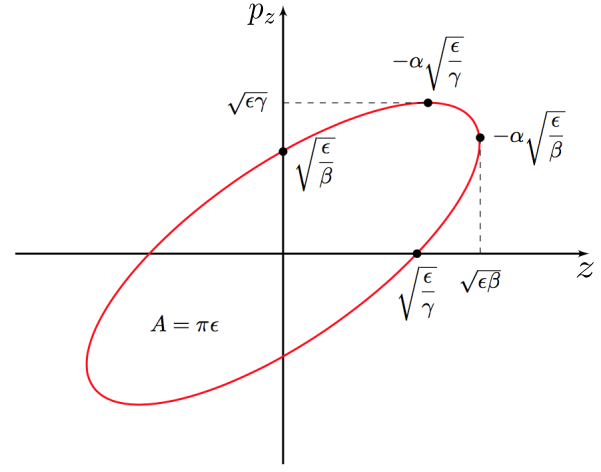
\includegraphics[width = 0.75\linewidth]{Figures/Beam_Dynamics_Theory/phase_space.png}
    \caption{Phase space ellipse in the transverse \((z, z^{\prime})\) plane, where \(z\) represents either transverse coordinate \(x\) or \(y\).}
    \label{figure:phase_space_ellipse}
    \end{center}
\end{figure}

According to the Liouville theorem the phase space volume, the ellipse area \(A\), is a constant in a closed system.
When accelerating the beam this theorem no longer holds true and the geometric emittance \(\varepsilon\) will decrease as the beam energy increases.
One can then construct the \intro{normalized emittance}, which is invariant with beam energy, based on the relativistic beta and gamma:

\begin{equation}
    \varepsilon_z^{\mathrm{norm}} = \beta_{\mathrm{rel}} \gamma_{\mathrm{rel}} \varepsilon_z \text{ .}
    \label{equation:normalized_emittance}
\end{equation}

When referring to the emittance of a specific particle one uses the term \intro{single particle emittance}.
The \intro{action} \(J_z\) is related to the single particle emittance by:

\begin{equation}
    2 J_z = \varepsilon_z \text{ .}
    \label{equation:single_particle_action}
\end{equation}

The state of particles in phase space can be fully characterized by the action variable \(J_z\) and the corresponding phase variable \(\phi_z\) seen above. 
Different particles in the beam will have different single particle emittances and will undergo betatron oscillations of varying amplitudes.
For a Gaussian shaped beam the transverse beam size is:

\begin{equation}
    \sigma_z = \sqrt{\beta_z \varepsilon_z^{\mathrm{beam}}} \text{ ,}
    \label{equation:gaussian_beam_transverse_beam_size}
\end{equation}
with \(\varepsilon_z^{\mathrm{beam}}\) the beam emittance, typically defined the emittance corresponding to a \(1 \sigma\) amplitude of the Gaussian charge distribution.
In the case of more general particle distributions an alternative definition of the beam emittance is often used~\cite{CERN:Muller:Beam_Matter_Covariance_Matrix_Emittance, CERN:Buon:CAS_Beam_Phase_Space_Emittance}:

\begin{equation}
    \varepsilon_z^{\mathrm{rms}} = \sqrt{\left\langle z \right\rangle^{2} \left\langle z^{\prime} \right\rangle^{2} - \left\langle zz^{\prime} \right\rangle^{2}} \text{ .}
    \label{equation:beam_emittance_general}
\end{equation}

The phase space trajectory of a particle depends on the Twiss parameters \(\alpha(s)\), \(\beta(s)\), and \(\gamma(s)\).
One can remove this dependency by performing a coordinate transformation to the \intro{Courant-Snyder coordinates}~\cite{BOOK:Bazzani:Normal_Form_Approach_Betatron_Motion}, defined as:

\begin{equation}
    \begin{+pmatrix}[cells={r}]
        \hat{z} \\
        \hat{z}^{\prime}
    \end{+pmatrix}
    =
    \begin{+pmatrix}[cells={r}]
        \frac{1}{\sqrt{\beta_z}} & \frac{\alpha_z}{\sqrt{\beta_z}} \\
        0 & \sqrt{\beta_z}
    \end{+pmatrix}
    \begin{+pmatrix}[cells={r}]
        z \\
        z^{\prime}
    \end{+pmatrix} \text{ ,}
    \label{equation:physical_to_courant_snyder_coordinates}
\end{equation}
where the Courant-Snyder coordinates are denoted by \^{}.
The same transformation is valid for \((z, p_z)\) to \((\hat{z}, \hat{p}_z)\) coordinates.
In this new system particles follow circular trajectories in phase space.
\Cref{figure:phase_space_linear_physical_normalized_coordinates} provides an illustrative representation of phase space in both physical and normalized coordinates for an accelerator with linear elements only.
In the new representation, the elliptical phase space is transformed into a simpler circular phase space where the motion is described by simple rotations, fully described by and depending only on the action and angle variables \((J_z, \phi_z)\).

\begin{figure}[!hbt]
    \begin{center}
    \begin{subfigure}[b]{0.45\textwidth}
        \begin{center}
        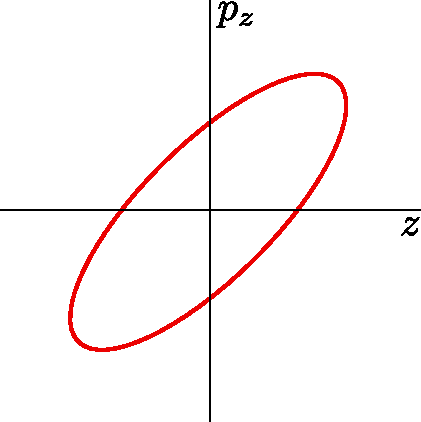
\includegraphics[width=\textwidth]{Figures/Beam_Dynamics_Theory/phase_space_linear_physical.pdf}
        \caption{Physical coordinates.}
        \label{fig:phase_space_physical}
        \end{center}
    \end{subfigure}
    \hfill
    \begin{subfigure}[b]{0.45\textwidth}
        \begin{center}
        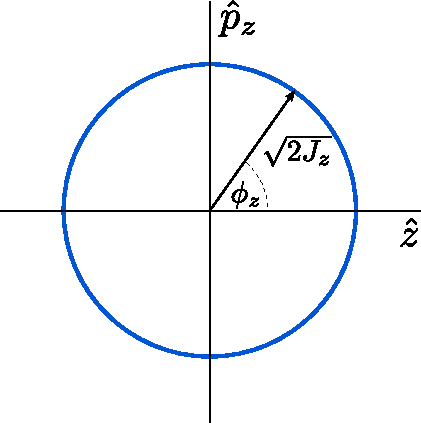
\includegraphics[width=\textwidth]{Figures/Beam_Dynamics_Theory/phase_space_linear_normalized.pdf}
        \caption{Normalized coordinates.}
        \label{fig:phase_space_normalized}
        \end{center}
    \end{subfigure}
    \caption{Illustrative representation of phase-space in physical coordinates (left) and normalized coordinates (right) for an accelerator with linear elements only. Courtesy of F. Carlier~\cite{PHD:Carlier}.}
    \label{figure:phase_space_linear_physical_normalized_coordinates}
    \end{center}
\end{figure}

\subsection{Chromatic Effects}
\label{subsection:chromatic_effects}

Until now, it was assumed that all particles had the intended design momentum \(p_{0}\).
Naturally, in practice particles withing the beam have a distribution in energy and momentum.
For a particle with a momentum \(p \neq p_{0}\) one defines and uses the \intro{relative momentum deviation} \(\delta_p\):

\begin{equation}
    \delta_p = \frac{p - p_0}{p_0} = \frac{\Delta p}{p_0} \text{ .}
    \label{equation:momentum_deviation}
\end{equation}

Such momenta offsets introduce \intro{chromatic errors} in the beam dynamics.
Effects and parameters depending on \(\delta_p\) are called \intro{chromatic effects}.

From the definition of the magnetic rigidity in \cref{equation:magnetic_rigidity}, it follows that particles of different momenta will have different local radii of curvature when going through dipoles and therefore follow different orbits along the machine.
The deviation of an off-momentum particle orbit from that of the synchronous particle is defined by the \intro{dispersion function} \(D(s)\).
Its contribution to a particle's orbit in a region of non-zero dispersion is described by:

\begin{equation}
    \Delta z_{\mathrm{dispersion}} = D_z(s) \delta_p \text{ .}
    \label{equation:dispersion_contribution_to_orbit}
\end{equation}
\bigbreak

Off-momentum particle positions scale linearly with dispersion, and in its presence \cref{equation:hill_solution} is extended to~\cite{BOOK:Wiedemann:Particle_Accelerator_Physics}:

\begin{equation}
    z(s) = \sqrt{\varepsilon_z \beta_z(s)} \cos \left( \phi_z(s) + \phi_{z, 0} \right) + D_z(s) \delta_p \text{ .}
    \label{equation:hill_solution_with_dispersion}
\end{equation}

Another chromatic parameter is the \intro{chromaticity} \(Q_z^{\prime}\), which describes the tune shift \(\Delta Q_z\) with particle momentum by:

\begin{eqnarray}
    Q^{\prime}_z = \frac{\Delta Q_z}{\delta_p} \text{ .}
    \label{equation:chromaticity_definition}
\end{eqnarray}

The effective focusing strength of quadrupoles, which is inversely proportional to the momentum, differs for off-momentum particles.
The change of focusing strength due to energy deviation is:

\begin{equation}
	\Delta k_{1} = - \dfrac{e}{p^2} \dfrac{d B_{y}}{d x} \Delta p = -k_{1} \delta_p \text{ .}
    \label{equation:quadrupole_focusing_strength_deviation_from_dispersion}
\end{equation}

This quadrupole error results in a tune shift proportional to the energy offset:

\begin{equation}
	\Delta Q = \dfrac{1}{4 \pi} \int \beta(s) \Delta k_{1}(s) ds = \left[ - \frac{1}{4 \pi} \int \beta(s) k_{1}(s) ds \right] \delta_p \text{ .}
    \label{equation:tune_shift_from_dispersion}
\end{equation}

The natural chromaticity of a linear lattice can then be approximated by~\cite{CAS:Guiducci:Chromaticity}:

\begin{equation}
    Q_z^{\prime} \approx -\frac{1}{4 \pi} \oint \beta_z(s) K_z \mathrm{d}s \text{ .}
    \label{equation:natural_chromaticity_approximation}
\end{equation}

%----------------------------------------------------------------------------------------

\section{Non-Linear Magnetic Multipoles}
\label{section:non_linear_magnetic_multipoles}

Magnetic fields of sextupolar and higher order are called \intro{non-linear} magnetic fields.
While only dipolar and quadrupolar magnetic fields are considered in the linear approximation, non-linear magnetic fields are present in most accelerators.
They can be introduced by design or by the presence of flaws in lower order magnets, the latter having the potential to seriously disrupt the beam.

The order of a multipole is labeled \(n\), with the convention that \(n = 1\) corresponds to a magnetic dipole, \(n = 2\) to a quadrupole, \(n = 3\) a sextupole, etc.
The magnetic field of a multipole of order \(n\) is given by:

\begin{equation}
    \begin{aligned}
    B_y(x, y, s) + i B_x(x, y, s) & = \sum_{n=1}^{\infty} \left[ B_n(s) + i A_n(s) \right] (x + i y)^{n-1} \text{ ,} \\
    B_n(s)                        & = \left. \frac{1}{(n - 1) !} \frac{\partial^{n - 1} B_y}{\partial x^{n - 1}} \right|_{(0,0,s)} \text{ ,} \\
    A_n(s)                        & = \left. \frac{1}{(n - 1) !} \frac{\partial^{n - 1} B_x}{\partial x^{n - 1}} \right|_{(0,0,s)} \text{ .} 
    \end{aligned}
    \label{equation:multipole_expansion}
\end{equation}

Here \(B_n(s)\) and \(A_n(s)\) are the normal and skew multipole coefficients, respectively, where a skew magnet of order \(n\) is rotated by \(\pi / (2 n)\) with respect to its normal counterpart.
Starting from the Hamiltonian equations:

\begin{equation}
    \dfrac{d \vec{p_z}}{d t} = - \frac{\partial \mathcal{H}}{\partial \vec{z}} \text{ ,} \quad \quad \quad \dfrac{d \vec{z}}{d t} = \frac{\partial \mathcal{H}}{\partial \vec{p_z}} \text{ ,}
    \label{equation:hamiltonian_equations}
\end{equation}

The Hamiltonian for the transverse planes for a multipole of order \(n\) is given by \cref{equation:hamiltonian_multipole_order_n}~\cite{PHD:Tomas, PHD:Franchi}:

\begin{equation}
    \mathcal{H} = \frac{q}{p} \operatorname{Re} \left[ \left( B_n +i A_n \right) \frac{(x + i y)^n}{n} \right] \text{ .}
    \label{equation:hamiltonian_multipole_order_n}
\end{equation}

In the linear regime, the Hamiltonian may then be written as:

\begin{equation}
    \mathcal{H} = \frac{1}{2} p_x^2 + \frac{1}{2} p_y^2 + \frac{1}{2} K(s) x^2 - \frac{1}{2} K(s) y^2 \text{ ,}
    \label{equation:hamiltonian_linear_lattice}
\end{equation}
where \(K(s)\) describes the variation of focusing strength around the ring.
More generally, if the Hamiltonian for a normal multipole of order \(n\) is labeled \(N_n\) and that of a skew multipole of order \(n\) is labeled \(S_n\), then~\cite{PHD:Maclean, PHD:Persson}:

\begin{equation}
    \begin{aligned}
        N_n & \propto \operatorname{Re} \left[(x + i y)^n \right] \\
            & \propto \operatorname{Re} \left[ \sum_{k=0}^n \left(
                \begin{array}{l}
                    n \\
                    k
                \end{array} \right) 
            i^k \beta_x^{\frac{n-k}{2}} \beta_y^{\frac{k}{2}} \left(\sqrt{2 J_x} \cos \phi_x \right)^{n-k} \left( \sqrt{2 J_y} \cos \phi_y \right)^k \right] \text{ ,}
    \end{aligned}
    \label{equation:hamiltonian_prop_normal_multipoles}
\end{equation}

\begin{equation}
    \begin{aligned}
        S_n & \propto \operatorname{Im} \left[(x + i y)^n \right] \\
            & \propto \operatorname{Im} \left[ \sum_{k=0}^n \left(
                \begin{array}{l}
                    n \\
                    k
                \end{array} \right) 
            i^k \beta_x^{\frac{n-k}{2}} \beta_y^{\frac{k}{2}} \left(\sqrt{2 J_x} \cos \phi_x \right)^{n-k} \left( \sqrt{2 J_y} \cos \phi_y \right)^k \right] \text{ .}
    \end{aligned}
    \label{equation:hamiltonian_prop_skew_multipoles}
\end{equation}

The powering of non-linear magnets and the presence of magnetic errors can have a significant impact on the beam dynamics.
Geometric errors can also contribute to the presence of non-linear components.

For instance, when a particle does not pass through the magnetic center of an element it will see not only the primary field component but also perturbations of all lower orders to that of the traversed element~\cite{BOOK:Wiedemann:Particle_Accelerator_Physics}.
This effect is called \intro{feed-down} and can be introduced by misalignment of lattice elements, which would cause the closed orbit to deviate from the ideal one and the beam to pass off-axis in magnets.

Should that happen with a sextupole, for instance, the beam would experience a sextupolar field but also encounter quadrupolar and dipolar components.
The rotational misalignment of elements is also a concern, as rotation a purely normal or skew multipole results in the beam experiencing a combination of both normal and skew fields.

%----------------------------------------------------------------------------------------

\section{Non-Linear Formalism and Resonance Driving Terms}
\label{section:non_linear_formalism_and_rdts}

The material below is inspired from~\cite{PHD:Tomas, PHD:Franchi,PHD:Maclean, PHD:Persson} where some aspects of it may be found in more details.
For the curious reader, a very thourough approach to normal forms can be found in~\cite{PHD:Carlier} and~\cite{PRAB:Franchi:First_Simultaneous}.

\subsection{Non-Linear Transfer Maps}
\label{subsection:non_linear_transfer_maps}

As introduced in \cref{equation:one_turn_map}, the dynamics of a circular accelerator can be parametrized in terms of \intro{transfer maps} relating final to initial phase space coordinates.
This approach is described in~\cite{BOOK:Bazzani:Normal_Form_Approach_Betatron_Motion, JMP:Forest:Hamiltonian_Free_Description_Single_Particle_Dynamics}.
While the transfer map of a linear element is described by a matrix, that of a non-linear element is itself described by the exponential \intro{Lie operator} \(e^{-:f:}\) defined as~\cite{BOOK:Wolski:Beam_dynamics}:

\begin{equation}
    \begin{aligned}
        e^{-:f:} g          &= g + \left[f, g\right] + \frac{1}{2} \left[f, \left[f, g \right] \right] + \ldots \text{ ,} \\
        \left[ f, g \right] &= \sum_i \frac{\partial f}{\partial q_i} \frac{\partial g}{\partial p_i} - \frac{\partial f}{\partial p_i} \frac{\partial g}{\partial q_i} \text{ ,}
    \end{aligned}
    \label{equation:lie_operator}
\end{equation}
where \(q_i\) and \(p_i\) are the canonical coordinates and momenta, respectively.
Here \(\left[ f, g \right]\) is the \intro{Poisson bracket} of \(f\) and \(g\).
When including non-linear sources, the one-turn map introduced in \cref{equation:one_turn_map} becomes:

\begin{equation}
    \mathrm{M_{OTM}} =e^{-:h_N:} e^{-:h_{N-1}:} \ldots e^{-:h_2:} e^{-:h_1:} R \text{ ,}
    \label{equation:one_turn_map_non_linear}
\end{equation}
where \(R\) is a matrix describing the linear dynamics of the machine, and the \(h_i\) terms represent the thin kick Hamiltonians of the non-linear elements in the accelerator.
\break

Relevant properties of the exponential Lie operator can be found in~\cite{PHD:Tomas, PHD:Franchi}, one of which being that the product of exponential Lie operators can be expressed as another exponential Lie operator following the \emph{Baker–Campbell–Hausdorff} theorem~\cite{BOOK:Hall:Lie_Group_Algebra_Representations}.
The one-turn map becomes:

\begin{equation}
    \mathrm{M_{OTM}} = e^{-:h:} R \text{ ,}
    \label{equation:Campbell_Baker_Hausdorff_theorem}
\end{equation}
in which, in case the \(h_n\) are small, \(h\) can be approximated as:
\begin{equation}
    h = \sum_{n=1}^N h_n + \sum_{n, m<n}^N \left[ h_m, h_n \right] + \ldots \text{ .}
    \label{equation:h_thin_kick_approximation}
\end{equation}

Using only the first order in \(h_n\), the thin kick \(h\) can be expressed in expanded terms using the action and angle variables according to:

\begin{equation}
    h = \sum_{jklm} h_{jklm} \left( 2 J_x \right)^{\frac{j+k}{2}} \left( 2 J_y \right)^{\frac{l+m}{2}} e^{i \left[ \left(j-k\right) \left(\phi_x - \phi_{x,0} \right) + \left(l-m\right) \left(\phi_y - \phi_{y,0} \right) \right]} \text{ ,}
    \label{equation:h_thin_kick_expansion}
\end{equation}
with \(h_{jklm}\) being the \intro{Hamiltonian coefficient} encompassing the contribution of all multipoles of order \(n = j + k + l + m\). 
\todo{The derivation for the result of \cref{equation:h_thin_kick_expansion} can be found in \cref{appendix:hamiltonian_derivation}.}

A multipole of order \(n = j + k + l + m\) gives rise to terms \(\propto x^{j+k} y^{l+m}\) in the Hamiltonian.
In the case of a skew quadrupole (\(n=2\)) for example, one will see terms in the Hamiltonian \(\propto xy\), meaning a contribution to \(h_{1010}\), \(h_{1001}\), \(h_{0110}\) and \(h_{0101}\).

\subsection{Normal Form, Resonance Driving Terms and Resonances}
\label{subsection:normal_form_and_rdt}

Due to the presence of non-linear sources the linear invariant \(J_z\) introduced in \cref{subsection:phase_space_ellipse} is no longer a constant.
This leads to the phase space trajectory in normalized, or Courant-Snyder, coordinates no longer describing a circle.
An example of this situation is given in \cref{figure:phase_space_third_order_resonance}, where the phase space trajectories of \num{200} particles are shown in normalized coordinates when exciting a third order resonance.

\begin{figure}[!htb]
    \begin{center}
    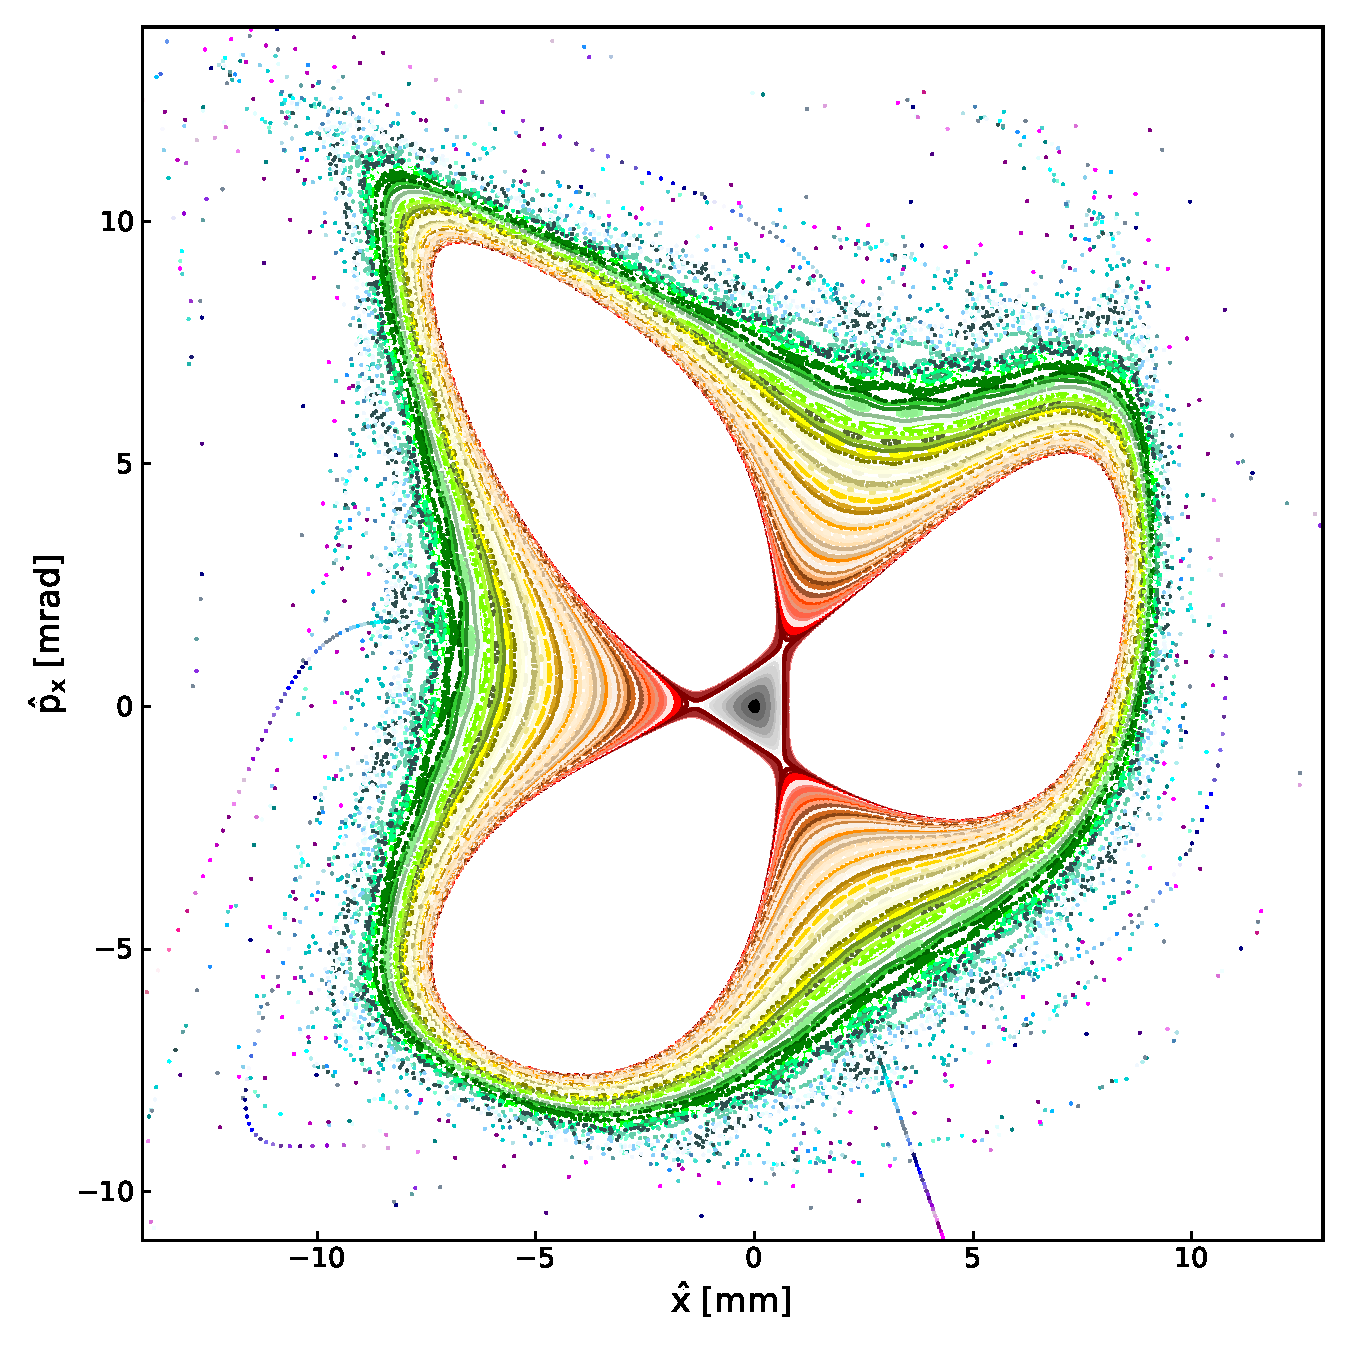
\includegraphics[width = 0.9\linewidth]{Figures/Beam_Dynamics_Theory/phase_space_third_order_resonance.pdf}
    \caption{Phase space in normalized coordinates from tracking \num{200} particles in a simple FODO-based lattice, when exciting a third order resonance. Points of each color corresponds to the trajectory of a given particle.}
    \label{figure:phase_space_third_order_resonance}
    \end{center}
\end{figure}

One may wish to create a new transformation, akin to that to normalized coordinates, that would allow describing betatron motion in phase space by a pure rotation in the presence of non-linear sources.
The change of coordinates is represented by a similarity transformation of the one turn map, written as~\cite{PHD:Tomas}:

\begin{equation}
    e^{-:F:} e^{:h:} R e^{:F:} \text{ ,}
    \label{equation:normal_form_transformation}
\end{equation}
where \(F\) is the \intro{generating function} of the transformation.
The coordinates resulting from the transformation are called \intro{normal form coordinates}.
The different coordinate systems are illustrated in \cref{figure:phase_space_non-linear_physical_normalized_normal_form_coordinates}.

\begin{figure}[!hbt]
    \begin{center}
    \begin{subfigure}[b]{0.30\textwidth}
        \begin{center}
        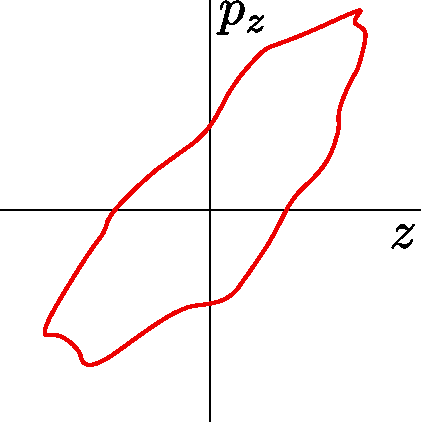
\includegraphics[width=\textwidth]{Figures/Beam_Dynamics_Theory/phase_space_nonlinear_physical.pdf}
        \caption{Physical coordinates.}
        \label{fig:phase_space_physical_non-linear}
        \end{center}
    \end{subfigure}
    \hfill
    \begin{subfigure}[b]{0.30\textwidth}
        \begin{center}
        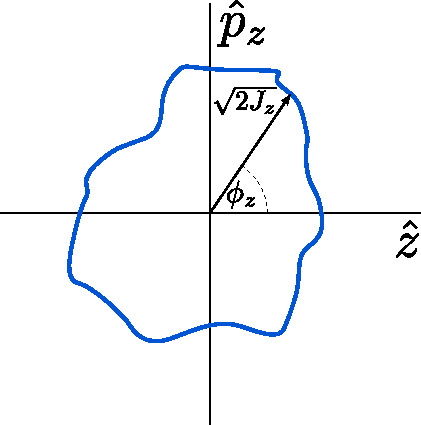
\includegraphics[width=\textwidth]{Figures/Beam_Dynamics_Theory/phase_space_nonlinear_normalized.pdf}
        \caption{Normalized coordinates.}
        \label{fig:phase_space_normalized_non-linear}
        \end{center}
    \end{subfigure}
    \hfill
    \begin{subfigure}[b]{0.3805\textwidth}
        \begin{center}
        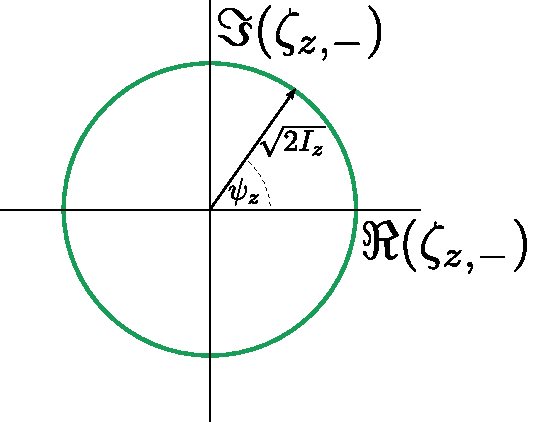
\includegraphics[width=\textwidth]{Figures/Beam_Dynamics_Theory/phase_space_nonlinear_normal_form.pdf}
        \caption{Normal form coordinates.}
        \label{fig:phase_space_normal_form_non-linear}
        \end{center}
    \end{subfigure}
    \caption{Illustrative exagerated representations of phase space in the three different coordinate systems: physical (left), normalized (middle) and normal form (right) coordinates. Courtesy of F. Carlier~\cite{PHD:Carlier}.}
    \label{figure:phase_space_non-linear_physical_normalized_normal_form_coordinates}
    \end{center}
\end{figure}

The generating function of the transformation \(F\) contains a large portion of the information describing the non-linear dynamics, and a new non-linear invariant \(I_z\) can be introduced. 
Similarly to \(h\) in \cref{equation:h_thin_kick_expansion}, the generating function \(F\) can be expanded in terms of the normal form coordinates according to~\cite{PHD:Franchi}:

\begin{equation}
    F = \sum_{jklm} f_{jklm} \left( 2 I_x \right)^{\frac{j+k}{2}} \left(2 I_y \right)^{\frac{l+m}{2}} e^{i \left[ (j-k) \left( \psi_x - \psi_{x_0} \right) + (l-m) \left( \psi_y - \psi_{y_0} \right) \right]} \text{ ,}
    \label{equation:generating_function_expansion}
\end{equation}
where \((I_z, \psi_z)\) are to normal form coordinates what \((J_z, \phi_z)\) are to normalized coordinates.
The \(f_{jklm}\) coefficients are related to the \(h_{jklm}\) terms by:

\begin{equation}
    f_{jklm} = \frac{h_{jklm}}{1 - e^{i 2 \pi \left[ \left(j-k\right) Q_x + \left(l-m\right) Q_y \right]}} \text{ .}
    \label{equation:resonance_driving_terms}
\end{equation}

From \cref{equation:resonance_driving_terms} one can see that the \(f_{jklm}\) coefficients diverge for certain values of the tunes.
Specifically, divergence happens when the following relation is satisfied:

\begin{equation}
    \left(j-k\right) Q_x + \left(l-m\right) Q_y = p \quad \quad \text { where } j, k, l, m, p \in \mathcal{Z} \text{ .}
    \label{equation:resonance_condition}
\end{equation}

A divergence of the \(f_{jklm}\) terms leads to a divergence of the transformation to normal form coordinates, which generally indicates an unclosed phase space trajectory due to a \intro{resonance} in the beam motion.
The condition in \cref{equation:resonance_condition} corresponds to situations where particles lie on resonant frequencies, typically causing their amplitudes to grow unbounded by the dynamics.
Therefore the \(f_{jklm}\) terms are called \intro{resonance driving terms} (RDTs).

For this reason, the tune is one of the single most important design parameters in synchrotrons.
The chosen operational transverse tunes of a synchrotron are known as its \intro{working point}, and should be chosen carefully in order to avoid resonances.
Resonances up to order \(n = 5\) are shown in \cref{figure:tune_diagram_fifth_order}, with lines of different orders differentiated from one another.

\begin{figure}[!htb]
    \begin{center}
    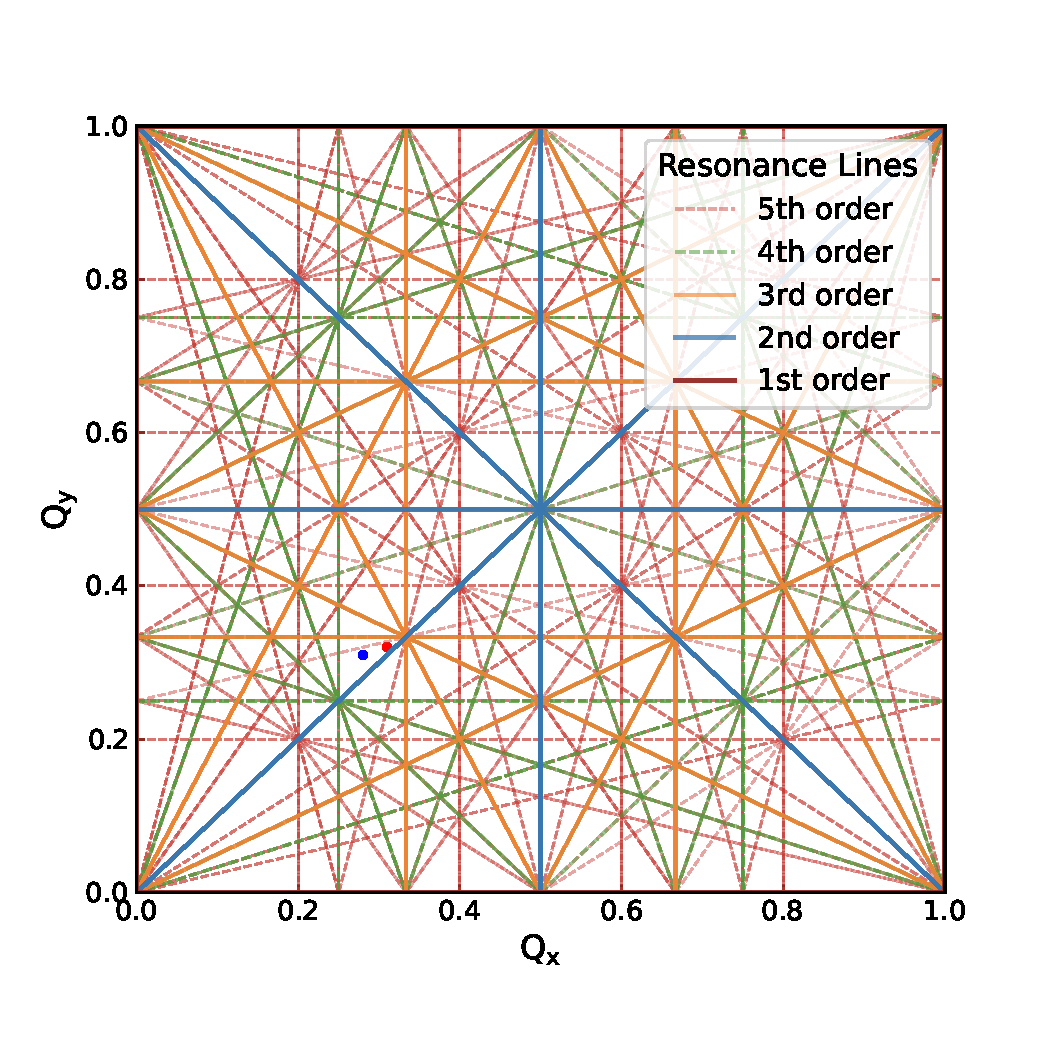
\includegraphics[width = 0.9\linewidth]{Figures/Beam_Dynamics_Theory/tune_diagram_fifth_order_with_working_points.pdf}
    \caption{Tunes diagram showing resonance lines up to order \(n = 5\). The LHC working points are indicated by the two dots: in \textcolor{wpblue}{blue} for injection tunes and \textcolor{wpred}{red} for collision tunes.}
    \label{figure:tune_diagram_fifth_order}
    \end{center}
\end{figure}

Commonly, the label of a given resonance is \(\left( n_1, n_2 \right)\), where \(n_1 = \left( j - k \right)\) and \(n_2 = \left( l - m \right)\).
Every generating function term \(f_{jklm}\), and equivalently every Hamiltonian term \(h_{jklm}\), is associated with a resonance.

The resonance driving terms vary in amplitude through the machine as they depend on local multipole strength of contributing sources.
Characteristically, the \(f_{jklm}\) terms show abrupt jumps at the location of relevant sources.

\todo{Maybe a figure of RDTs accross a known machine to illustrate?}

\subsection{Resonance Basis and Normal Form Coordinates}

The normalized Courant-Snyder coordinates \(\left( \hat{z}, \hat{p}_z \right)\) are related to the action and angle variables \(\left( J_z, \phi_z \right)\) by:

\begin{equation}
    \begin{aligned}
        \hat{z}   &= \sqrt{2 J_z} \cos \left( \phi_z - \phi_{z_0} \right) \text{ ,} \\
        \hat{p}_z &= - \sqrt{2 J_z} \sin \left( \phi_z - \phi_{z_0} \right) \text{ .}
    \end{aligned}
    \label{equation:normalized_courant_snyder_coordinates_from_action_angle}
\end{equation}

One can define the \intro{resonance basis} \(\left( h_x^{+}, h_x^{-}, h_y^{+}, h_y^{-} \right)\) by the relation:

\begin{equation}
    h_z^{\pm} = \hat{z} \pm i \hat{p}_z = \sqrt{2 J_z} e^{\mp i \left( \phi_z + \phi_{z_0} \right)} \text{ .}
    \label{equation:resonance_basis_definition}
\end{equation}

The transformation to the \kl{normal form coordinates} \(\left( \zeta_x^{+}, \zeta_x^{-}, \zeta_y^{+}, \zeta_y^{-} \right)\) is expressed as:

\begin{equation}
    \zeta_z^{\pm} = \sqrt{2 I_z} e^{\mp i \left( \psi_z + \psi_{z_0} \right)} = e^{-:F:} h_z^{\pm} \text{ .}
    \label{equation:transformation_to_normal_form_coordinates_from_h_pm}
\end{equation}
where \((I_u, \psi_u)\) are the terms introduced in \cref{equation:generating_function_expansion}.

By construction of the transformation, the one-turn map in normal form coordinates is an amplitude dependent rotation.
It follows that the motion of these coordinates as a function of the turn number is then given by:

\begin{equation}
    \zeta_u^{\pm}(N) = \sqrt{2 I_u} e^{\mp i \left( 2 \pi \nu_u N + \psi_{u_0} \right)} \text{ ,}
    \label{equation:normal_form_N_turn_expression}
\end{equation}
with \(\nu_u\) the transverse tunes.
The inverse transformation from the new action and angle variables to the Courant-Snyder variables is written, to first order, as:

\begin{equation}
    h_u^{-} = e^{:F:} \zeta_u^{-} \simeq \zeta_u^{-} + \left[ F, \zeta_u^{-} \right] \text{ .}
    \label{equation:inverse_transformation_normal_form-to_courant_snyder_coordinates}
\end{equation}

Using \cref{equation:normal_form_N_turn_expression} and \cref{equation:inverse_transformation_normal_form-to_courant_snyder_coordinates}, the linearly normalized coordinates can be expressed after \(N\) turns as~\cite{CERN:Bartolini:Normal_Form_Tracking_Beam_Data}:

\begin{equation}
    \begin{aligned}
        h_x^{-}(N) & = \sqrt{2 I_x} e^{i \left( 2 \pi \nu_x N - \psi_{x_0} \right)} \quad - \\
        & \quad 2 i \sum_{jklm} j f_{jklm} \left( 2 I_x \right)^{\frac{j+k-1}{2}} \left( 2 I_y \right)^{\frac{l+m}{2}}   e^{i \left[ (1-j+k) \left( 2 \pi \nu_x N-\psi_{x_0} \right) + (m-l)   \left( 2 \pi \nu_y N - \psi_{y_0} \right) \right]} \\
        h_y^{-}(N) & = \sqrt{2 I_y} e^{i \left( 2 \pi \nu_y N - \psi_{y_0} \right)} \quad - \\
        & \quad 2 i \sum_{jklm} l f_{jklm} \left( 2 I_x \right)^{\frac{j+k}{2}}   \left( 2 I_y \right)^{\frac{l+m-1}{2}} e^{i \left[ (k-j)   \left( 2 \pi \nu_x N-\psi_{x_0} \right) + (1-l+m) \left( 2 \pi \nu_y N - \psi_{y_0} \right) \right]} \text{ .}
    \end{aligned}
    \label{equation:linearly_normalized_coordinates_after_N_turns}
\end{equation}


\Cref{figure:coordinate_transformations} shows a schematic of the different transformations and changes to the one-turn map.
While one can calculate the evolution of the Courant-Snyder coordinates by applying the map \( \mathcal{M} \), the approach is complicated to solve.
Solving the one-turn map for the next turn is best done by performing a transformation to normal form coordinates \(\zeta_{u}^{\pm}\) using the generating function \(F\), applying the amplitude dependent rotation map \(R\), and transforming back to Courant-Snyder coordinates.
These calculations are in practice simpler than the former method, and conserve non-linearities.

\begin{figure}[!htb]
    \begin{center}
    \begin{tikzpicture}
        \matrix (m) [matrix of math nodes,row sep=4em,column sep=4em,minimum width=2em]{
            \left(\hat{u}, \hat{p}_u\right)_N    &    \left(\hat{u}, \hat{p}_u\right)_{N+1} \\
            \zeta_{u_N}^{\pm}{}                  &    \zeta_{u_{N+1}}^{\pm}{}  \\
        };
        \path[-stealth]
        (m-1-1) edge node [above] {\( \mathcal{M} \)} (m-1-2)
        (m-1-1) edge node [left] {\( e^{:-F:} \)} (m-2-1)
        (m-2-1.east|-m-2-2) edge node [below] {\( e^{-:h:} R \)} (m-2-2)
        (m-2-2) edge node [right] {\( e^{:F:} \)} (m-1-2);
    \end{tikzpicture}
    \caption{Illustration of the coordinate transformations and change of the one-turn map. This diagram reads from Courant-Snyder coordinates at turn \(N\) in the top left, and shows both paths to reach the Courant-Snyder coordinates at turn \(N+1\) in the top right.}
    \label{figure:coordinate_transformations}
    \end{center}
\end{figure}

\subsection{Spectral Contribution}
\label{subsec:spectral_contribution}

Each term in the summations of \cref{equation:linearly_normalized_coordinates_after_N_turns} corresponds to a certain mode in the beam motion and contributes to a specific frequency in the spectrum of the motion~\cite{PHD:Bengtsson}.
Said spectrum may be determined by a frequency analysis of the turn-by-turn beam position monitor data, through means of a Fourier transform.
In this spectrum, an RDT \(f_{jklm}\) at a specific location in the machine contributes to lines in the horizontal and vertical spectra according to~\cite{PHD:Bengtsson,PRAB:Franchi:Emittance_Sharing_Coupling}:

\begin{equation}
    \begin{aligned}
        H(1-j+k, m-l) &= 2 j \abs{f_{jklm}} \left( 2 I_x \right)^{\frac{j+k-1}{2}} \left( 2 I_y \right)^{\frac{l+m}{2}} \text{ ,}\\
        V(k-j, 1-l+m) &= 2 l \abs{f_{jklm}} \left( 2 I_x \right)^{\frac{j+k}{2}} \left( 2 I_y \right)^{\frac{l+m-1}{2}} \text{ ,}
    \end{aligned}
    \label{equation:rdt_contribution_to_spectrum_line}
\end{equation}
where in the parentheses multiples of the fractional tunes are given.
For example, \(H(0,1)\) indicates an observed line at \(1 \times Q_y\) in the horizontal spectrum.
\Cref{figure:example_spectrum} shows an example of a spectrum from a measurement at the LHC, where the main lines are highlighted.

\begin{figure}[!htb]
    \begin{center}
    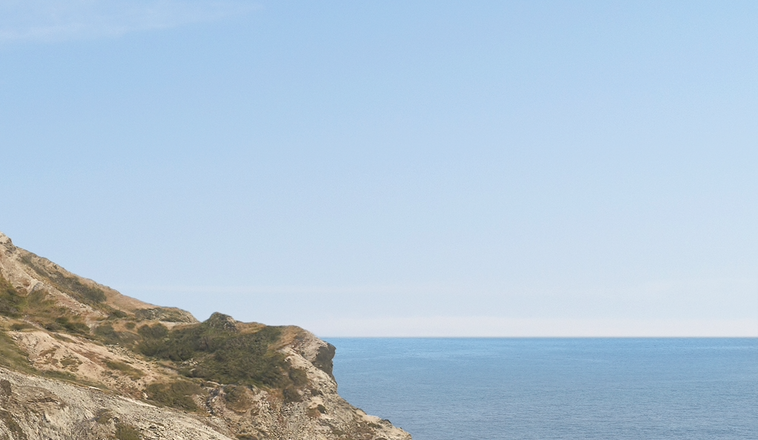
\includegraphics[width = 0.3\linewidth]{Figures/placeholder.png}
    \caption{\todo{Include a plot of a spectrum from an LHC measurement? Something out of omc3, maybe the one in my sextupolar contribution to ampdet ATS note.}}
    \label{figure:example_spectrum}
    \end{center}
\end{figure}

In principle the \(\abs{f_{jklm}}\) may be determined by a comparison of the amplitude of various spectral lines.
In practice, some additional considerations need to be taken, as decoherence of a kicked beam can lead to a reduction in the amplitude of the spectral lines observed, or the fact that the contributions of different RDTs might not be distinct.
More details are given in \cref{chapter:lhc_omc}.

%----------------------------------------------------------------------------------------

\section{Betatron Coupling}
\label{section:betatron_coupling}

When the betatronic motion of particles in transverse planes are independent of each other, they are said to be \intro{uncoupled}.
In particle colliders such as the LHC this is the desired behaviour.
When these motions share a dependency, they are said to be \intro{coupled}, and one refers to this phenomenon as \intro{betatron coupling}.
The transverse motions of particles in an accelerator may couple due to a variety of factors, with solenoid and skew quadrupole fields being the primary sources of linear coupling.

In the LHC the main contribution to coupling comes from unwanted skew quadrupolar fields.
These mostly arise from normal quadrupoles mounted with a rotation error with respect to the longitudinal axis, but also from field imperfection from other magnets and feed-down from higher order magnets.
An example of a skew quadrupole is given in \cref{figure:skew_quadrupole}.

\begin{figure}[!htb]
    \begin{center}
    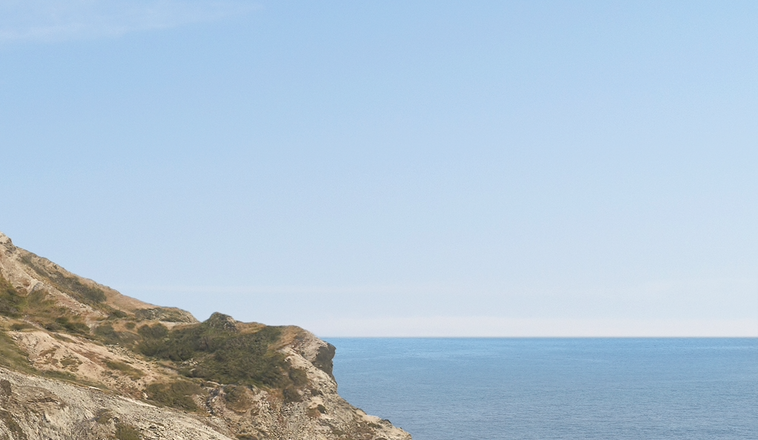
\includegraphics[width = 0.5\linewidth]{Figures/placeholder.png}
    \caption{\todo{Illustration of a skew quadrupole and its magnetic field lines.}}
    \label{figure:skew_quadrupole}
    \end{center}
\end{figure}

Betatron coupling needs to be kept under control as it can perturb the tune feedback systems and push tunes into resonances, or simply lead to a reduction in the dynamic aperture~\cite{PA:Ripken:Impact_Linear_Coupling_Nonlinear_Dynamics}.

\subsection{Parametrization of Betatron Coupling}
\label{subsection:parametrization_of_betatron_coupling}

There are different ways to parametrize coupled motion in a particle accelerator, the two most common being the Edwards-Teng~\cite{IEEE:Edwards:Parametrization_Linear_Coupled_Motion} and Mais-Ripken~\cite{AIP:Willeke:Methods_Beam_Optics} parametrizations.
For coupled motion a dependency between the horizontal and vertical planes is introduced, and as such the transverse motions can no longer be described by two independent \(2 * 2\) matrices.
Instead, it is described by a \(4 \times 4\) matrix \(\hat{\mathbf{M}}\):

\begin{equation}
    \hat{\mathbf{M}} = \left(
        \begin{array}{ll}
            \mathbf{P} & \mathbf{p} \\
            \mathbf{q} & \mathbf{Q}
    \end{array} \right) \text{ ,}
    \label{equation:coupled_motion_matrix}
\end{equation}
where \(\mathbf{P}\), \(\mathbf{p}\), \(\mathbf{q}\) and \(\mathbf{Q}\) are \(2 \times 2\) matrices.
In the absence of betatron coupling, it follows that \(\mathbf{p}\) and \(\mathbf{q}\) are \num{0}.

In the Edwards-Teng parametrization presented in~\cite{IEEE:Edwards:Parametrization_Linear_Coupled_Motion}, the linear coupling is described by a symplectic rotation \(\mathbf{R}\) of \(\hat{\mathbf{M}}\) into its normal modes form \(\overline{\mathbf{M}}\), as shown in \cref{equation:edwards_teng_parametrization}.
In this frame the motion is decoupled.

\begin{equation}
    \overline{\mathbf{M}} = \left(
        \begin{array}{cc}
            \mathbf{X} & 0 \\
            0 & \mathbf{Y}
    \end{array} \right) = \mathbf{R} \hat{\mathbf{M}} \mathbf{R}^{-1} \text{ .}
    \label{equation:edwards_teng_parametrization}
\end{equation}

Edwards and Teng characterized the transformation \(\mathbf{R}\) by the symplectic matrix:

\begin{equation}
    \mathbf{R} =\left(
        \begin{array}{cc}
            \mathbf{I} \cos \theta & -\mathbf{K}^{-1} \sin \theta \\
            \mathbf{K} \sin \theta & \mathbf{I} \cos \theta
    \end{array} \right) \text{ ,}
    \label{equation:edwards_teng_rotation_matrix}
\end{equation}
where \(\mathbf{I}\) is the \(2 \times 2\) unit matrix and \(\mathbf{K}\) is a \(2 \times 2\) symplectic matrix, such that \(det(\mathbf{K}) = 1\).
The coupled motion may then be described by the uncoupled Twiss parameters seen in \cref{subsection:equations_of_motion_and_twiss_parameters}, together with the elements of matrix \(\mathbf{K}\) and Teng's angle of rotation \(\theta\).
In the case that \(\theta = 0\), the matrix \(\mathbf{R}\) is the identity matrix and as a result it will not rotate any of the modes: this corresponds to uncoupled motion.

The Edwards-Teng parameterization is used in the MAD-X~\cite{CODE:MADX_guide} code when handling coupled motion.
In MAD-X the relevant parameters are \(\alpha_{x, y}\), \(\beta_{x, y}\), \(\mu_{x, y}\), \(\gamma_{x, y}\) and \(r_{11}\), \(r_{12}\), \(r_{21}\), \(r_{22}\), where \(r_{11} \ldots r_{22}\) correspond to the elements of \(\mathbf{K}\) multiplied by \(\tan(\theta)\).

The approach of Mais and Ripken was developed in~\cite{REPORT:Ripken:AllGerman} and is more accessible in~\cite{AIP:Willeke:Methods_Beam_Optics, REPORT:Borchardt:Calculation_Beam_Envelopes}.
It defines so-called \intro{Ripken parameters} \(\alpha_{kj}\), \(\beta_{kj}\) and \(\gamma_{kj}\), where \(k = 1 \ldots 3\) refers to the plane (\(x, y, \ldots\)) and the index \(j\) refers to the eigenmodes, that are accurate in the presence of coupling.
In the coupled case, all \(\beta_N\) are non-zero and \(\beta_{11}, \beta_{22}\) are distinctively different from \(\beta_x, \beta_y\), respectively.
The relations linking these new parameters to the Twiss parameters can be found in~\cite{IOP:Lebedev:Betatron_Motion_Coupling}.
% The relations linking these new parameters to the Twiss parameters is~\cite{IOP:Lebedev:Betatron_Motion_Coupling}:

% \begin{equation}
%     \begin{aligned}
%     \beta_x &= \frac{\beta_{11}}{1-u} \text{ ,} \quad \alpha_x = \frac{\alpha_{11}}{1-u}, \\
%     \beta_y &= \frac{\beta_{21}}{1-u} \text{ ,} \quad \alpha_y = \frac{\alpha_{21}}{1-u},
%     \end{aligned}
%     \label{equation:ripken_to_twiss_parameters}
% \end{equation}
% where \(\sin \phi = \pm \sqrt{u}\) is the rotation of the x-y plane. When φ = 0 there is no coupling and β x = β 11
The Mais-Ripken parameterization is the basis of the Polymorphic Tracking Code's (PTC~\cite{CODE:Schmidt_Forest:PTC}) handling of coupled dynamics. 

\subsection{Coupled Motion}
\label{subsection:coupled_motion}

In the first order, according to \cref{equation:resonance_condition}, linear coupling drives the two resonances \(Q_x + Q_y = p\) and \(Q_x - Q_y = p\), with \(p \in \mathcal{Z}\).
These are respectively called the \intro{sum and difference resonances}, and in their vicinity the beam dynamics are heavily influenced.
To higher order betatron coupling may also give stationary terms in the Hamiltonian (a tune shift), driving the \(2 Q_x\) and \(2 Q_y\) resonances, but these effects are typically negligible.

The impact of linear coupling on the beam motion has been studied through Hamiltonian perturbation theory~\cite{PHREV:Guignard:Betatron_Coupling_Radiation,BOOK:Wiedemann:Particle_Accelerator_Physics} and through the normal form / resonance driving term formalism~\cite{PHD:Franchi}.

As the transverse tunes approach the difference resonance, the emittance is described by:

\begin{equation}
    \varepsilon_x + \varepsilon_y = \mathrm{const} \text{ ,}
    \label{equation:coupled_emittances_difference_resonance}
\end{equation}
and as the resonance is approached the beam motion may not become unstable.
Instead, there is a periodic exchange of emittance between the transverse planes, which leads to a beating in the betatron oscillation amplitudes.

The relation between the \intro{unperturbed tunes} \(Q_{x,y}\) and the \intro{coupled tunes} \(Q_{1,2}\) is given by~\cite{CAS:Bryant:Theory_Weak_Betatron_Coupling}:

\begin{equation}
    \begin{aligned}
        Q_1 &= Q_x- \frac{\Delta}{2} + \frac{\sqrt{\Delta^2 + \abs{C^{-}}}}{2} \text{ ,} \\
        Q_2 &= Q_y+ \frac{\Delta}{2} - \frac{\sqrt{\Delta^2 + \abs{C^{-}}}}{2} \text{ ,}
    \end{aligned}
    \label{equation:unperturbed_tunes_to_coupled_tunes}
\end{equation}
with \(\Delta\) being the unperturbed fractional tune split and \AbsCminus the linear coupling coefficient, a parameter describing the strength of the coupling.

When \(\Delta \gg \abs{C^{-}}\), away from the resonance, the observed oscillations modes \(Q_{1,2}\) are almost identical to the uncoupled horizontal and vertical tunes \(Q_{x,y}\).
When the tunes are moved closer together, approching the difference resonance (\(\Delta \rightarrow 0\)), the perturbed tunes are forced apart by the coupling and a minimal tune separation \(\Delta Q_{\mathrm{min}}\) can be observed.
The \AbsCminus of \cref{equation:unperturbed_tunes_to_coupled_tunes}, named the \intro{closest tune approach}, corresponds this separation.
\Cref{figure:closest_tune_approach} shows an illustration of the phenomenon in the vicinity of the resonance, where both the unperturbed (dashed) and coupled (colored) fractional tunes are plotted against the uncoupled tune split.
% TODO: adapt this plot to have Q_{1,2} instead of Q_{x,y}
\begin{figure}[!htb]
    \begin{center}
    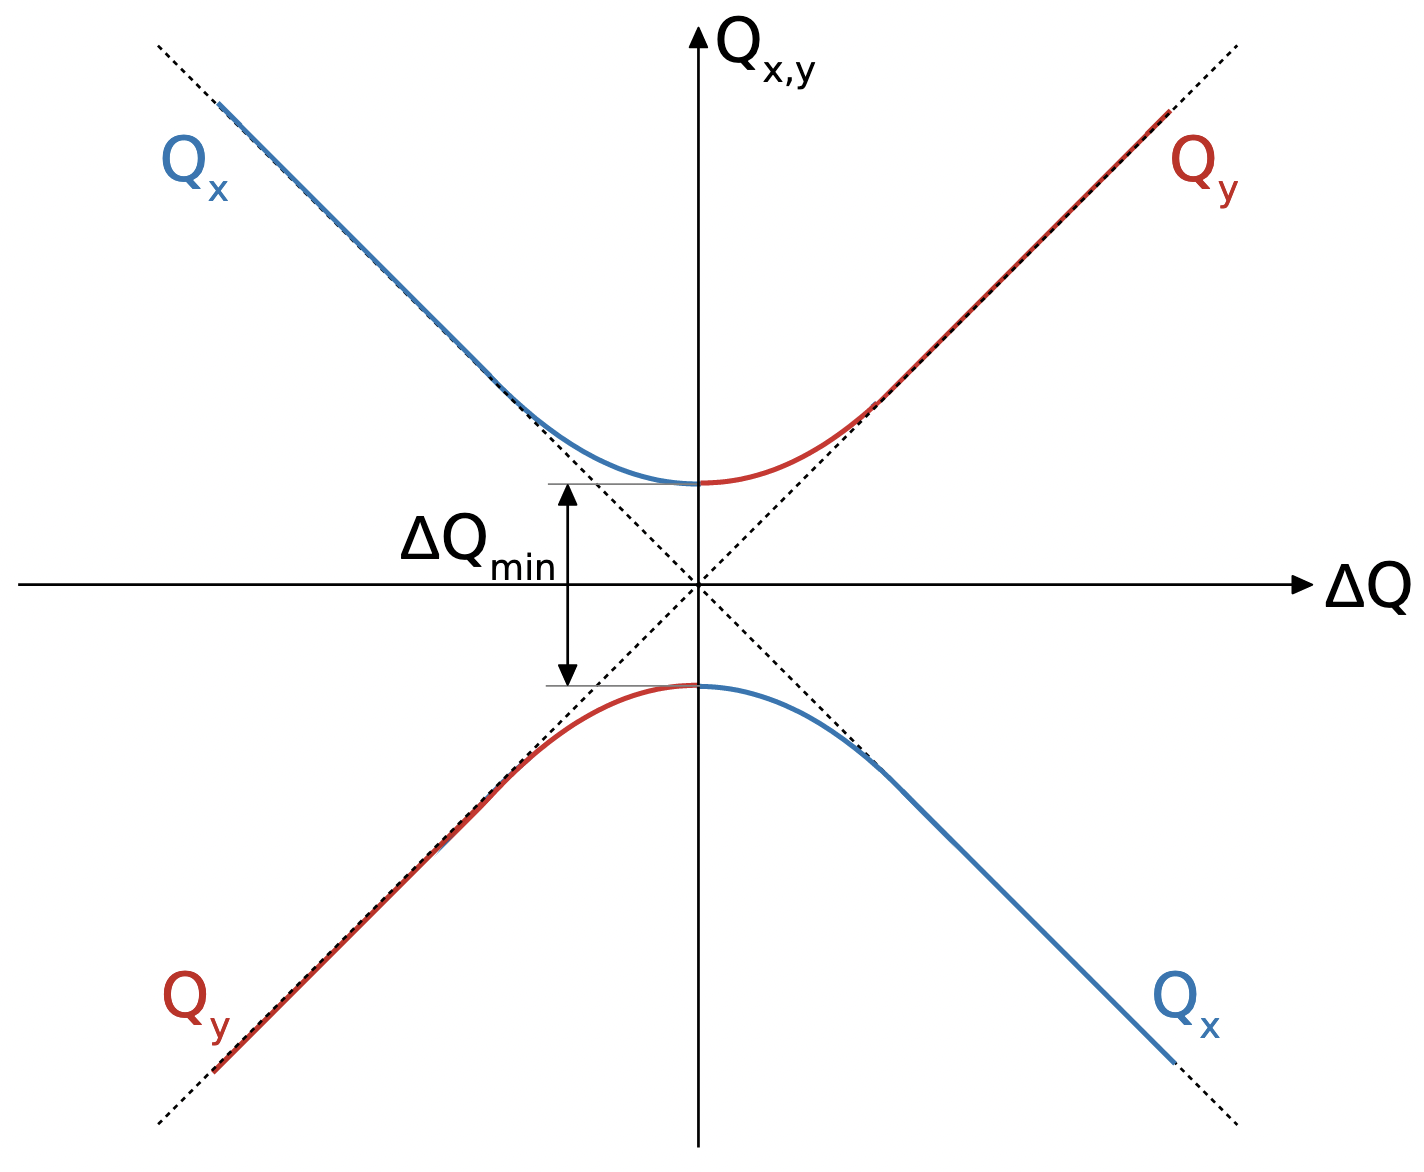
\includegraphics[width = 0.9\linewidth]{Figures/Beam_Dynamics_Theory/closest_tune_approach_schematic.png}
    \caption{Illustration of coupled and uncoupled fractional tunes versus the uncoupled tune split. Courtesy of J. Keintzel~\cite{PHD:Keintzel}.}
    \label{figure:closest_tune_approach}
    \end{center}
\end{figure}

On the other hand, when approaching the sum resonance the emittances follow:

\begin{equation}
    \varepsilon_x - \varepsilon_y = \mathrm{const} \text{ .}
    \label{equation:coupled_emittances_sum_resonance}
\end{equation}

This resonance allows for unstable motion as only the difference in emittance is constrained.
Therefore, it is common to choose a working point far from the sum resonance.
In the LHC, the working points (visible on \cref{figure:tune_diagram_fifth_order}) are set such that the linear coupling is dominated by the difference resonance: \((Q_x, Q_y) = (0.28 \text{,} 0.31)\) at injection and \((Q_x, Q_y) = (0.31 \text{,} 0.32)\) for squeezed beams and collisions\footnote{The LHC working point is actually slightly more diverse and will be discussed in more details in the next chapter.}.

\subsection{Linear Coupling Resonance Driving Terms}
\label{subsection:measurement_coupling_rdts}

Linear coupling in the LHC is dominated by the contribution of skew quadrupole fields, which lead to terms \(\propto xy\) in the Hamiltonian.
According to the resonance relation of \cref{equation:resonance_condition} and as seen in \cref{subsection:coupled_motion}, this gives rise to the resonance driving terms \(f_{1001}\) and \(f_{0110}\), which correspond to the \(Q_x - Q_y = p\) difference resonance; and \(f_{1010}\) which corresponds to the \(Q_x + Q_y = p\) sum resonance.
The \(f_{1001}\) and \(f_{0110}\) describe the same dynamics but the former is for the horizontal plane while the latter is for the vertical plane.
Since they describe the same dynamics it is custom to label both of them as \(f_{1001}\), which is a convention used throughout this thesis.

It was mentioned in \cref{subsection:coupled_motion} that the LHC working point is selected to be close to the stable difference resonance, and as a consequence in the LHC the \(\abs{f_{1001}}\) dominates relative to the \(\abs{f_{1010}}\).
These RDTs can be expressed as a function of the uncoupled lattice parameters at the location of both the coupling-contributing elements and the observation point \(s\) as~\cite{PHREV:Guignard:Betatron_Coupling_Radiation}:

\begin{equation}
    \begin{aligned}
        f_{1001}(s) &= - \frac{1}{4 \left(1 - e^{2 \pi i \left(Q_x - Q_y \right)}\right)} \sum_l k_l \sqrt{\beta_x^l \beta_y^l} e^{i \left(\Delta \phi_x^{s l} - \Delta \phi_y^{s l}\right)} \text{ ,} \\
        f_{1010}(s) &= - \frac{1}{4 \left(1 - e^{2 \pi i \left(Q_x + Q_y \right)}\right)} \sum_l k_l \sqrt{\beta_x^l \beta_y^l} e^{i \left(\Delta \phi_x^{s l} + \Delta \phi_y^{s l}\right)} \text{ ,}
    \end{aligned}
    \label{equation:coupling_rdts_from_skew_quads}
\end{equation}
where \(k_l\) is the \(l\)th integrated skew quadrupole strength, \(\beta_{x,y}^{l}\) are the \(\beta\)-functions at the location of the \(l\)th skew quadrupole, \(Q_{x,y}\) are the horizontal and vertical tunes, and \(\Delta \phi_{x,y}^{s l}\) are the phase advances from the \(l\)th skew quadrupole to the observation point at the longitudinal coordinate \(s\).
The summation is done over all contributing skew quadrupoles.

These resonance driving terms can be related to the strength of the coupling \(\Delta Q_{\mathrm{min}}\), and as such the \(\abs{C^{-}}\) can be expressed in relation to the \(f_{1001}\) RDT.
In~\cite{PHD:Franchi} this relation was established as:

\begin{equation}
    \abs{C^{-}} \approx 4 \Delta \frac{1}{N} \sum_{i=1}^N \abs{f_{1001}}_i \text{ ,}
    \label{equation:deltaqmin_from_f1001_franchi}
\end{equation}
where the summation is done over the \(N\) observation points, and \(\Delta\) is the fractional tune split.
A more accurate relation was established in~\cite{PRAB:Persson:Improved_Control_Betatron_Coupling}, which is:

\begin{equation}
    \abs{C^{-}} = \abs{\frac{4 \Delta}{2 \pi R} \oint d s f_{1001} e^{-i \left(\phi_x - \phi_y \right) + i s \Delta / R} } \text{ ,}
    \label{equation:deltaqmin_from_f1001}
\end{equation}
where the dependence of variables on the position \(s\) was omitted for clarity.

In~\cite{PHREV:Guignard:Betatron_Coupling_Radiation} the equations of motion are solved perturbatively under the influence of a weak skew quadrupole strength \(j(s)\).
Assuming that the machine is close to the difference coupling resonance \(\Delta = Q_x - Q_y \rightarrow 0\), the \(\abs{C^{-}}\) can be approximated as:

\begin{equation}
    \abs{C^{-}} = \frac{1}{2 \pi} \abs{ \oint ds \sqrt{\beta_x(s) \beta_y(s)} j(s) e^{-i \left( \phi_x - \phi_y \right) + i \frac{s \Delta}{R}} } \text{ ,}
    \label{equation:deltaqmin_guignard}
\end{equation}
where \(s\) is the position around the ring, \(\beta_{x,y}\) are the horizontal and vertical \(\beta\)-functions, \(\phi_{x,y}\) are the phase advances and \(R\) is the radius of the machine.

\todo{I think I would like to mention something about~\cite{PRAB:Calaga:Coupling_Merging_Hamiltonian_Matrix_Approaches} before ending this section.}
% \todo{Can refer to~\cite{PRAB:Franchi:First_Simultaneous} for table with many RDTs.}

%----------------------------------------------------------------------------------------

\section{Luminosity}
\label{section:luminosity}

The LHC machine being a particle collider, it is operated to produce collisions between two counter-rotating beams and to produce data for High Energy Physics experiments.
As the studied interactions coming from these collisions are rare, a substantial volume of statistics is required. 
Naturally, the performance of the machine is then described by the number of collisions provided to experiments as well as the center-of-mass energy of these collisions.

As a figure of merit for the number of collisions the \intro{luminosity} is used.
The \intro{instantaneous luminosity} \(\mathcal{L}\) is the proportional factor between the number of events per unit of time \(dR / dt\) and the process cross-section \(\sigma_{\mathrm{cross}}\):

\begin{equation}
    \dfrac{dR}{dt} = \mathcal{L} \sigma_{\mathrm{cross}} \text{ .}
    \label{equation:instantaneous_luminosity_definition}
\end{equation}

The instantaneous luminosity is given in units of inverse barns per second (\unit{\per\barn\per\second}), where \(\left[ b \right] = \) \qty{1e-24}{\per\square\centi\meter}.
For a collider with Gaussian beams, it can be expressed as~\cite{CERN:Herr:Concept_Luminosity}:

\begin{equation}
    \mathcal{L} = \frac{f_{\mathrm{rev}} N_1 N_2}{4 \pi \sigma_x \sigma_y} S \text{ ,}
    \label{equation:luminosity_gaussian_beams}
\end{equation}
where \(f_{\mathrm{rev}}\) is the revolution frequency of particle bunches, \(N_1\) and \(N_2\) are the number of particles in each beam, and \(\sigma_{x,y}\) are the transverse beam sizes at the interaction points.
\(S\) is the luminosity reduction factor and depends on the crossing of the beams: crossing angles, orbit offset, non-zero dispersion or even the hourglass effect will impact its value.

For Gaussian bunches colliding with a \intro{crossing angle} \(\theta\), where \(\sigma_s \gg \sigma_{x,y}\) and neglecting other contributions, the luminosity reduction factor is approximated by~\cite{CERN:Herr:Concept_Luminosity}:

\begin{equation}
    S \approx \frac{1}{\sqrt{1 + \left( \frac{\theta}{2} \frac{\sigma_s}{\sigma_x} \right)^2}} \text{ ,}
    \label{equation:luminosity_reduction_factor}
\end{equation}

As seen in \cref{equation:gaussian_beam_transverse_beam_size} the beam sizes directly depend on the \(\beta\)-function at the IP, \betastar, which then defines the collider's performance from the point of view of the optics.
Indeed, the smaller the \(\beta^{\ast}\) the smaller the beam sizes, and the more collisions will be produced per bunch crossing. 
The downside to small beam sizes, which is a direct consequence of the \kl{Louiville theorem}, is that they cause large beam divergence.
This is illustrated by the evolution of the \(\beta\)-function in the drift space around the IP:

\begin{equation}
    \beta(s) = \beta^{\ast} + \frac{s^2}{\beta^{\ast}}
    \label{equation:betafunction_drift_space}
\end{equation}
where here \(s\) is the distance from the IP.
As usually collisions are made to happen in the centre of large particle detectors, there is no space near the IP to place quadrupoles to keep the \(\beta\)-functions low, hence the presence of a substantial drift space.
The experimental insertion regions will be discussed in more details in \cref{section:lhc_lattice}.

The \intro{integrated luminosity}, the accumulated luminosity over a given period of time, is given by:

\begin{equation}
    \mathcal{L}_{\mathrm{int}} = \int_{t_1}^{t_2} \mathcal{L} \mathrm{d}t \text{ ,}
    \label{equation:integrated_luminosity}
\end{equation}

The integrated luminosity is usually in units of \unit{\per\femto\barn} \(=\) \qty{1e39}{\per\square\centi\meter}.
The total number of collisions, or events, over said time period is then:

\begin{equation}
    \mathrm{N_{events}} = \mathcal{L}_{\mathrm{int}} \sigma_{\mathrm{cross}} \text{ .}
    \label{equation:total_number_collisions}
\end{equation}

Throughout luminosity production, the instantaneous luminosity naturally decreases as more and more particles are lost to collisions~\cite{PRES:Hostettler:LHC_Lumi_Lifetime}.
Any particle losses happening before colliding the beams will lead to a reduction of the initial \(N_{1,2}\) and of the resulting integrated luminosity of the given fill.\\

Luminosity production requires a good control of the linear optics, both for the quality of the optics themselves but also for a smooth and safe operation.
Many non-linear contributions may also influence the dynamics away from the linear regime, leading to a deterioration of the dynamics and, down the line, the luminosity.
Therefore for a particle collider like the LHC a good control of all effects influencing the beam dynamics is required, and methods to both measure and correct any deviations from the ideal machine are a necessity.
An overview of these will be given in \cref{chapter:lhc_omc}

%----------------------------------------------------------------------------------------